%%%%%%%%%%%%%%%%%%%%%%%%%%%%%%%%%%%%%%%%%%%%%%%%%%%%%%%%%%%%
%%% Virtual Zebrafish v60 — Technical Report
%%%%%%%%%%%%%%%%%%%%%%%%%%%%%%%%%%%%%%%%%%%%%%%%%%%%%%%%%%%%
\documentclass[11pt,a4paper]{article}

\usepackage[margin=2.5cm]{geometry}
\usepackage{amsmath,amssymb,amsfonts}
\usepackage{graphicx}
\usepackage{booktabs}
\usepackage{hyperref}
\usepackage{cleveref}
\usepackage{caption}
\usepackage{subcaption}
\usepackage{float}
\usepackage{algorithm}
\usepackage{algorithmic}
\usepackage{tikz}
\usetikzlibrary{arrows.meta, positioning, shapes, calc, fit}
\usepackage{xcolor}
\usepackage{enumitem}
\usepackage{multirow}

\definecolor{forage}{RGB}{34,139,34}
\definecolor{flee}{RGB}{220,50,50}
\definecolor{explore}{RGB}{50,100,220}

\title{%
  \textbf{A Biologically Grounded Virtual Zebrafish:\\
  From Retinal Sampling to Active Inference Policy Selection}\\[8pt]
  \large Technical Report --- Zebrafish SNN v60 (Steps 1--25)
}
\author{Hae-Jeong Park\\
  Department of Nuclear Medicine \& Cognitive Science\\
  Yonsei University College of Medicine, Seoul, Korea\\
  \texttt{parkhj@yonsei.ac.kr}
}
\date{\today}

\begin{document}
\maketitle

%===================================================================
\begin{abstract}
We present a spiking neural network (SNN) model of the larval zebrafish brain
that implements the full perception--action loop: from binocular retinal
sampling through tectal processing and predictive coding to locomotor output
with neuromodulatory control.
The model is developed in twenty-five progressive steps, each adding a
biologically motivated computational module.
Steps~1--6 establish visual tracking with precision adaptation, dopamine-based
reward prediction error, basal ganglia motor gating, optic tectum dynamics,
and cross-modal salience.
Steps~7--10 close the sensorimotor loop with autonomous locomotion,
genomic (evolutionary) pre-training, and Hebbian fine-tuning.
Steps~11--12 add object classification and classification-guided reactive
behavior.
Step~13 transitions from reactive to deliberative behavior via Expected Free
Energy (EFE)-based policy selection with working memory, implementing three
goal states---\textsc{forage}, \textsc{flee}, and \textsc{explore}.
Step~14 embeds the brain in a Gymnasium-compatible environment with energy
homeostasis, depth-shaded vision, obstacle collision physics, and a habit
network that consolidates stable EFE decisions into fast shortcut responses.
Step~15 adds a reinforcement learning critic that adapts EFE weights online
via temporal-difference error.
Step~16 introduces a variational autoencoder (VAE) world model with
associative memory and forward-simulation planning.
Step~17 implements hippocampal place cells with path integration, replay, and
spatial planning.
Step~18 adds allostatic interoception---predictive tracking of hunger,
fatigue, and stress that biases goal selection.
Step~19 provides a full evaluation suite comparing baseline, full-brain, and
place-cell configurations.
Step~20 introduces an amygdala fear circuit with persistent threat arousal,
flee energy cost asymmetry, and nonlinear hunger-driven foraging urgency.
Step~21 adds active-inference food prospection with line-of-sight
reachability scoring, olfactory heading cues, and retinal obstacle navigation.
Step~22 introduces a curriculum reinforcement learning framework with
progressive difficulty scaling.
Step~23 adds a sleep--wake cycle for memory consolidation with precision
freeze and fatigue recovery.
Step~24 completes the active inference architecture by replacing all
ground-truth environment reads with generative-model inference: a retinal
feature extractor, VAE-based threat decoder, interoceptive energy model,
and boundary-corrected path integration ensure the agent perceives only
through its own sensory channels.
Step~25 replaces single-compartment neurons with two-compartment
predictive coding cells featuring apical dendrite feedback and
goal-driven additive attention, with homeostatic gain control and
PE-driven anti-Hebbian feedback learning, reducing prediction error
64\% and improving survival from 100\% to 60\% catch rate.
All modules use biologically plausible local learning rules without
backpropagation through time.
In closed-loop simulations, the virtual zebrafish successfully forages for
food (3--6 items per 800-step episode), avoids predators, navigates around
rock formations, and explores its environment with goal-appropriate
behavioral modulation driven by interoceptive and exteroceptive signals.
\end{abstract}

\tableofcontents
\newpage

%===================================================================
\section{Introduction}\label{sec:intro}

Larval zebrafish (\textit{Danio rerio}, 5--7 days post-fertilization) offer a
unique model system: a vertebrate brain small enough for whole-brain calcium
imaging, yet complex enough to exhibit visually guided prey capture, predator
avoidance, and social behavior~\cite{ahrens2013,portugues2014}.

This report documents a computational model---\textbf{ZebrafishSNN\_v60}---that
recapitulates key neural circuits of the larval zebrafish using a hierarchy of
spiking neural network layers.
The model is built incrementally across twenty-four developmental steps, each
introducing one functional module.
The design philosophy is:
\begin{enumerate}[nosep]
  \item \textbf{Biological plausibility}: leaky integrator neurons, local
    Hebbian plasticity, no backpropagation through time.
  \item \textbf{Modularity}: each brain region (retina, optic tectum,
    pretectum, basal ganglia, thalamus) is an independent module.
  \item \textbf{Active inference}: behavior is driven by minimizing expected
    free energy over a small goal space.
  \item \textbf{Developmental curriculum}: modules are added and tested
    progressively, mirroring biological maturation.
\end{enumerate}

%===================================================================
\section{Model Architecture}\label{sec:arch}

\subsection{Overview}

The full processing pipeline is:
\[
  \underbrace{\text{Retina}}_{\text{800}\times 2}
  \;\xrightarrow{\text{topographic}}\;
  \underbrace{\text{OT}_{L/R}}_{\text{600}\times 2}
  \;\xrightarrow{\text{lateral inh.}}\;
  \underbrace{\text{OT}_F}_{800}
  \;\xrightarrow{\pi_\text{OT}}\;
  \underbrace{\text{PT}}_{400}
  \;\rightarrow\;
  \underbrace{\text{PC}_{per}}_{120}
  \;\xrightarrow{\pi_\text{PC}}\;
  \underbrace{\text{PC}_{int}}_{30}
  \;\rightarrow\;
  \begin{cases}
    \text{Motor} & (200) \\
    \text{Eye}   & (100) \\
    \text{DA}    & (50)
  \end{cases}
\]

A separate classification head branches from the bilateral retinal type
channels:
\[
  [\mathbf{L}_{400:},\; \mathbf{R}_{400:}] \;\xrightarrow{800 \to 64 \to 5}\;
  \text{class logits}.
\]

\subsection{Neuron Model: Two-Compartment Leaky Integrator}

Each layer uses a first-order discrete leaky integrator:
\begin{equation}\label{eq:twocomp}
  \mathbf{v}(t) = \tau\,\mathbf{v}(t-1) + (1-\tau)\,\bigl(\mathbf{x}(t)\,\mathbf{W}\bigr),
  \quad \tau = 0.8,
\end{equation}
where $\mathbf{W} \in \mathbb{R}^{n_{in}\times n_{out}}$ is initialized as
$0.01\,\mathcal{N}(0,1)$.
The effective time constant is $\tau/(1-\tau)=4$ steps.
In Step~25 (Section~\ref{sec:predictive_attention}), trainable layers are
upgraded to two-compartment predictive coding neurons with apical feedback
and attention modulation; the frozen topographic layers
OT$_\text{L}$/OT$_\text{R}$ retain this single-compartment form.

%===================================================================
\section{Sensory Processing}\label{sec:sensory}

\subsection{Binocular Retinal Sampling (Step 1)}

Each eye samples a $20\times 20$ angular grid (400 pixels) over a horizontal
field of view of $\pm 80^\circ$ and elevation range of $\pm 20^\circ$.
The left eye is centered at $\theta_{\text{head}} - 45^\circ$, the right at
$\theta_{\text{head}} + 45^\circ$.

Each pixel has two channels:
\begin{itemize}[nosep]
  \item \textbf{Intensity channel} with Gaussian foveation:
    \begin{equation}\label{eq:foveation}
      G(\alpha) = \exp\!\Bigl(-\frac{\alpha^2}{2\sigma^2}\Bigr),
      \quad \sigma = 12^\circ,
    \end{equation}
    where $\alpha$ is the azimuthal offset from eye center.
  \item \textbf{Type channel} (unfoveated) carrying entity identity:
    food$\,{=}\,1.0$, enemy$\,{=}\,0.5$, colleague$\,{=}\,0.25$,
    boundary$\,{=}\,0.12$, none$\,{=}\,0.0$.
\end{itemize}

Total retinal output per eye: $\mathbf{L}, \mathbf{R} \in [0,1]^{1\times 800}$.

\subsection{Tectal Topography}

Optic tectum weights are initialized with retinotopic Gaussian receptive
fields:
\begin{equation}\label{eq:topography}
  W_{ij} = \exp\!\Bigl(-\frac{(x_i^{in} - x_j^{out} - \delta)^2}{2\sigma_T^2}\Bigr),
  \quad \sigma_T = 0.10,
\end{equation}
where $\delta = -0.15$ (left) or $+0.15$ (right) implements nasotemporal shift.
Type channels receive $0.7\times$ the intensity-channel weight.

\subsection{Lateral Inhibition}

Winner-take-all competition between left and right OT channels sharpens the
bilateral contrast signal:
\begin{equation}\label{eq:latinh}
  \mathbf{o}_L^{out} = \mathbf{o}_L - \lambda\,\mathbf{o}_R,
  \quad
  \mathbf{o}_R^{out} = \mathbf{o}_R - \lambda\,\mathbf{o}_L,
  \quad \lambda = 0.25.
\end{equation}

\subsection{Retinal Turn Signal}

The basic turn signal is computed from intensity-channel asymmetry:
\begin{equation}\label{eq:turn}
  \text{turn} =
  \frac{\sum R_{1:400} - \sum L_{1:400}}
       {\sum R_{1:400} + \sum L_{1:400} + 10^{-8}}.
\end{equation}

%===================================================================
\section{Predictive Coding and Precision (Step 2)}\label{sec:precision}

\subsection{Free Energy}

At the tectal fusion level, free energy is computed as precision-weighted
prediction error:
\begin{equation}\label{eq:freeenergy}
  F = \tfrac{1}{2}\,\overline{\pi}_\text{OT}\,
      \bigl\|\mathbf{o}_\text{fused} - \mathbf{o}_F\,\mathbf{W}_{OTF}^\top\bigr\|^2,
\end{equation}
where $\overline{\pi}_\text{OT} = \text{mean}(\sigma(\boldsymbol{\gamma}_\text{OT}))$.

\subsection{Precision Units}

Each precision unit maintains a learnable logit $\boldsymbol{\gamma}$ with
output $\pi = \sigma(\boldsymbol{\gamma})$, updated as:
\begin{equation}\label{eq:precision}
  \Delta\gamma = \alpha_\pi\,(|\varepsilon| - \beta)
    - 0.05\,\nu\,\mathbb{1}[\nu > 0.03],
\end{equation}
where $|\varepsilon|$ is the mean absolute error, $\beta = 0.1$ is the target
error level, $\nu = ||\varepsilon|(t) - |\varepsilon|(t{-}1)|$ is the novelty
signal, and $\alpha_\pi = 0.05$.
Precision is clamped: $\gamma \in [-3, 3]$.

Two precision units operate at different hierarchical levels:
\begin{itemize}[nosep]
  \item $\pi_\text{OT}$ (800-dim): applied to fused OT output $\mathbf{o}_F$.
  \item $\pi_\text{PC}$ (120-dim): applied to perisomatic PC layer.
\end{itemize}

%===================================================================
\section{Neuromodulation}\label{sec:neuromod}

\subsection{Dopamine System (Step 3)}

The dopamine system models VTA/SNc dynamics with TD-style reward learning.

\paragraph{Pseudo-reward.}
\begin{equation}\label{eq:reward}
  r(t) = \exp\!\bigl(-|F_\text{vis}(t)|\bigr) + 0.5 \cdot n_\text{eaten}.
\end{equation}

\paragraph{Value learning and RPE.}
\begin{equation}\label{eq:td}
  \text{RPE}(t) = r(t) - V(t),
  \quad
  V(t{+}1) = \bigl(V(t) + \alpha_V\,\text{RPE}(t)\bigr)\cdot\delta_V,
\end{equation}
with $\alpha_V = 0.05$ and $\delta_V = 0.98$.

\paragraph{Dopamine level.}
\begin{equation}\label{eq:dopa}
  \text{DA}(t) = \sigma\!\bigl(\beta_\text{DA}\cdot\text{RPE}(t)\bigr) + \xi,
  \quad \xi \sim \mathcal{N}(0, 0.01),
\end{equation}
clamped to $[0, 1]$.
Baseline DA $= 0.5$ (neutral); $> 0.5$ signals reward, $< 0.5$ signals
aversion.

\paragraph{Bilateral valence.}
\begin{equation}\label{eq:valence}
\begin{aligned}
  v_L(t) &= (1{-}\delta_v)\,v_L(t{-}1) + 0.1\,(e_L - 0.5\,e_R), \\
  v_R(t) &= (1{-}\delta_v)\,v_R(t{-}1) + 0.1\,(e_R - 0.5\,e_L),
\end{aligned}
\end{equation}
where $e_{L/R} = \overline{o}_{L/R} - 0.5\,V$, $\delta_v = 0.02$.
Mean-subtracted and clamped to $[-0.5, 0.5]$.

\paragraph{Dopamine--precision coupling.}
\begin{equation}\label{eq:dopa_prec}
  \Delta\gamma_{\text{OT/PC}} \mathrel{+}= 0.008\,(\text{DA} - 0.5).
\end{equation}

\subsection{Cross-Modal Salience --- Thalamus (Step 6)}

The thalamic relay computes cross-modal salience (CMS):
\begin{equation}\label{eq:cms}
  \text{CMS}(t) = (1{-}\alpha_s)\,\text{CMS}(t{-}1) + \alpha_s
  \Bigl[\gamma_\Delta\,\frac{\Delta F_v + \Delta F_a}{2}
    + (1{-}\gamma_\Delta)\,|F_v - F_a|\Bigr],
\end{equation}
with $\gamma_\Delta = 0.6$, $\alpha_s = 0.1$.

CMS modulates downstream systems:
\begin{equation}\label{eq:cms_mod}
\begin{aligned}
  \beta_\text{DA}  &= 3.0\,(1 + 0.5\,\text{CMS}), &
  \sigma_\text{BG} &= \sigma_0\,(1 + 2.0\,\text{CMS}), \\
  \pi_\text{bias}  &= \pi\,(1 - 0.2\,\min(\text{CMS},1)).
\end{aligned}
\end{equation}

%===================================================================
\section{Motor Control}\label{sec:motor}

\subsection{Basal Ganglia Gating (Step 4)}

The basal ganglia implements action selection through switching dynamics:

\paragraph{Drive.}
$d = (v_R - v_L) + 0.3\,(\text{DA} - 0.5)$.

\paragraph{Momentum integration.}
\begin{equation}\label{eq:bg_momentum}
  p(t) = 0.65\,p(t{-}1) + 0.35\,d(t).
\end{equation}

\paragraph{State update with dopamine-gated leak.}
\begin{equation}\label{eq:bg_state}
  s(t) = s(t{-}1) + 0.3\,p(t)
    - \ell_\text{eff}\,s(t{-}1) + \sigma_\text{BG}\,\xi,
\end{equation}
where $\ell_\text{eff} = 0.10\,(1 + 0.5\,\max(0,\; 0.5 - \text{DA}))$.

\paragraph{Gate output.}
$g = \tanh(0.8\,s) \in [-1, 1]$.

\paragraph{Exploratory switching.}
With probability $p_\text{sw} = 0.12\,\sigma(5\,|\text{RPE}|)$, momentum
reverses sign, producing RPE-triggered saccadic switching.

\subsection{Optic Tectum Eye Control (Step 5)}

Continuous eye-movement dynamics integrating salience competition, free energy,
and BG gating:
\begin{equation}\label{eq:ot_eye}
\begin{aligned}
  \dot{v}_\text{eye} &= 0.35\bigl[\tanh(1.5(v_R{-}v_L)) - 0.15\,F + 0.12\,g\bigr]
                       - 0.35\,v_\text{eye}, \\
  e(t{+}1) &= e(t) + 0.2\,v_\text{eye}
              - 0.18\,(1{+}0.5\max(0, 0.5{-}\text{DA}))\,e(t).
\end{aligned}
\end{equation}

\subsection{Closed-Loop Locomotion (Step 7)}

The complete locomotor command:
\begin{equation}\label{eq:locomotion}
\begin{aligned}
  \theta(t{+}1) &= \theta(t) + 0.15\,\tilde{\tau} + 0.03\,g + 0.02\,e, \\
  v_\text{swim}  &= v_0\,s_\text{mod}\,(0.8 + 0.4\,\text{DA}), \\
  x(t{+}1)      &= x(t) + v_\text{swim}\cos\theta, \\
  y(t{+}1)      &= y(t) + v_\text{swim}\sin\theta,
\end{aligned}
\end{equation}
where $\tilde{\tau}$ is the smoothed, modulated turn signal, $v_0 = 1.5$,
and $s_\text{mod}$ is a goal-dependent speed multiplier.

%===================================================================
\section{Learning}\label{sec:learning}

\subsection{Genomic Pre-training (Step 8)}

Supervised learning mimics evolutionary pre-wiring of the motor pathway.
Training minimizes:
\begin{equation}\label{eq:genomic_loss}
  \mathcal{L} = \|\hat{\tau} - \tanh(2\alpha_\text{food})\|^2
    + 0.3\,\|\hat{\phi} - \alpha_\text{food}/\pi\|^2,
\end{equation}
where $\hat{\tau}$ is the decoded motor turn and $\hat{\phi}$ the predicted
eye angle.
Adam optimizer with $\text{lr}=0.005$, cosine annealing, gradient clipping at
1.0, for 120 epochs $\times$ 50 samples.

\subsection{Hebbian Fine-tuning (Step 10)}

RPE-gated Hebbian plasticity refines connections during foraging:
\begin{equation}\label{eq:hebbian}
  \Delta\mathbf{W} = \eta\,\text{RPE}\,\text{DA}\;
    (\mathbf{x}_\text{pre}^\top \mathbf{x}_\text{post}),
  \quad
  \mathbf{W} \leftarrow 0.9999\,\mathbf{W},
\end{equation}
with $\eta = 0.0005$.
Applied to OT fusion weights and motor output head.

\subsection{Object Classification (Step 11)}

A two-layer classifier (800$\to$64$\to$5) is trained on bilateral retinal type
channels using cross-entropy loss:
\begin{equation}\label{eq:cls_loss}
  \mathcal{L}_\text{cls} = -\sum_c y_c \log p_c,
  \quad
  p = \text{softmax}(\mathbf{W}_2\,\text{ReLU}(\mathbf{W}_1\,\mathbf{t}) + \mathbf{b}_2),
\end{equation}
where $\mathbf{t} = [\mathbf{L}_{400:},\;\mathbf{R}_{400:}]$.
Five classes: nothing, food, enemy, colleague, environment.
Trained for 150 epochs with $\text{lr} = 0.01$; achieves $> 80\%$ per-class
accuracy.

%===================================================================
\section{Reactive Behavior (Step 12)}\label{sec:reactive}

Classification probabilities directly modulate behavior:
\begin{equation}\label{eq:reactive}
\begin{aligned}
  a_\text{gain} &= 1.0 + 0.3\,p_\text{food}
    - 1.5\,\max(0,\; p_\text{enemy} - 0.6) + 0.15\,p_\text{colleague}, \\
  s_\text{mod} &= 1.0 + 0.2\,p_\text{food} + 0.6\,\max(0,\; p_\text{enemy} - 0.5), \\
  e_\text{mod} &= \max\!\bigl(0.2,\; 1.0 + 0.3\,p_\emptyset - 0.3\,(p_f + p_e)\bigr),
\end{aligned}
\end{equation}
where $a_\text{gain}$ is the approach gain (positive = approach, negative =
flee), $s_\text{mod}$ is the speed multiplier, and $e_\text{mod}$ is the
exploration multiplier.
The turn signal is modulated as $\tilde{\tau}_\text{mod} = \tau_\text{raw} \cdot a_\text{gain}$.

%===================================================================
\section{Active Inference Policy Selection (Step 13)}\label{sec:active}

Step~13 transitions from frame-by-frame reactive behavior to deliberative
goal selection via Expected Free Energy (EFE) minimization.

\subsection{Goal Space}

Three discrete goals: $\mathcal{G} = \{\textsc{forage},\; \textsc{flee},\;
\textsc{explore}\}$.

\subsection{Expected Free Energy}

For each goal $g_i$, the EFE combines epistemic (uncertainty-reducing) and
pragmatic (reward-seeking) terms:
\begin{equation}\label{eq:efe}
\boxed{
\begin{aligned}
  G_\textsc{forage}  &= 0.2\,\mathcal{U} - 0.8\,p_\text{food}
    + 0.2\,(0.5 - \text{DA}) + 0.15, \\
  G_\textsc{flee}    &= 0.1\,\text{CMS} - 0.8\,p_\text{enemy} + 0.40, \\
  G_\textsc{explore} &= 0.3\,\mathcal{U}
    - 0.5\,(p_\emptyset + p_\text{env})
    + 0.1\,\text{CMS} + 0.20,
\end{aligned}
}
\end{equation}
where $\mathcal{U} = 1 - \tfrac{1}{2}(\pi_\text{OT} + \pi_\text{PC})$ is the
model uncertainty.
Lower EFE indicates a more preferred goal.

Key design features:
\begin{itemize}[nosep]
  \item $G_\textsc{flee}$ has a high baseline ($+0.40$), ensuring it is only
    selected when $p_\text{enemy}$ is high.
  \item Dopamine modulates $G_\textsc{forage}$: low DA increases foraging drive.
  \item CMS (novelty) promotes both fleeing and exploring.
\end{itemize}

\subsection{Policy Posterior}

The posterior over goals uses a softmax with inverse temperature $\beta = 2.0$:
\begin{equation}\label{eq:posterior}
  \pi(g_i) = \frac{\exp(-\beta\,(G_i - G_\text{min}))}
                   {\sum_j \exp(-\beta\,(G_j - G_\text{min}))}.
\end{equation}

\subsection{Persistence and Emergency Override}

A timer-based persistence mechanism prevents goal flickering:
\begin{itemize}[nosep]
  \item Minimum persistence: 8 steps per goal episode.
  \item \textbf{Emergency override}: if $p_\text{enemy} > 0.7$, immediately
    switch to \textsc{flee} (biological fight-or-flight).
  \item \textbf{Context-sensitive early exit}: \textsc{flee} exits early after
    3 steps if $p_\text{enemy} < 0.2$; \textsc{forage} exits after 4 steps if
    $p_\text{food} < 0.15$.
  \item Re-selection uses $\arg\max \pi(g)$.
\end{itemize}

\subsection{Confidence (Meta-Precision)}

Entropy-based confidence provides a meta-level precision signal:
\begin{equation}\label{eq:confidence}
  \text{conf} = 1 - \frac{H(\boldsymbol{\pi})}{\ln 3},
  \quad
  H(\boldsymbol{\pi}) = -\sum_i \pi(g_i)\ln\pi(g_i).
\end{equation}

\subsection{Goal-to-Behavior Mapping}

\begin{table}[H]
\centering
\caption{Behavioral modulation by active goal.}
\label{tab:goal_behavior}
\begin{tabular}{lccc}
\toprule
Goal & $a_\text{gain}$ & $s_\text{mod}$ & $e_\text{mod}$ \\
\midrule
\textsc{forage}  & $1.0 + 0.5\,p_f\,c$ & $1.0 + 0.3\,p_f$   & 0.5 \\
\textsc{flee}    & $-(0.8 + 0.5\,p_e\,c)$ & $1.3 + 0.4\,p_e$ & 0.3 \\
\textsc{explore} & 0.8 & 0.9 & $1.5 + 0.5(1{-}c)$ \\
\bottomrule
\end{tabular}

\medskip
\small $p_f = p_\text{food}$, $p_e = p_\text{enemy}$, $c = \text{conf}$.
\end{table}

\subsection{Working Memory}

A 16-dimensional latent memory trace integrates classification, goal state,
and neuromodulatory context:
\begin{equation}\label{eq:latent}
  \mathbf{z}_t = [p_1,\ldots,p_5,\; g_1,g_2,g_3,\;
    \text{DA},\; \text{CMS},\; F,\; \pi_\text{OT},\; \pi_\text{PC},\;
    \bar{g}_1,\bar{g}_2,\bar{g}_3],
\end{equation}
where $\bar{g}$ is a decaying goal trace: $\bar{g}(t) = 0.9\,\bar{g}(t{-}1) + 0.1\,g(t)$.

Memory update:
\begin{equation}\label{eq:memory}
  \mathbf{m}(t) = (1 - \alpha_\text{eff})\,\mathbf{m}(t{-}1)\,d_\text{DA}
    + \alpha_\text{eff}\,\mathbf{z}_t,
\end{equation}
where $\alpha_\text{eff} = \text{clip}(\alpha/(1{+}\gamma\,s), 0.01, 0.3)$,
$d_\text{DA} = 1 + 0.2(\text{DA} - 0.5)$, and CMS modulates the effective
alpha: $\alpha_\text{eff} \leftarrow \alpha_\text{eff}(1 + 0.3\,\text{CMS})$.

%===================================================================
\section{Simulation Results}\label{sec:results}

Each step was validated with specific pass/fail criteria.
The figures referenced below are generated automatically by the test scripts.

\subsection{Step 1: Vision Pursuit}

A sinusoidally sweeping stimulus ($y = 60\sin(2\pi t/100)$, $T = 200$) tests
basic visual tracking.
The fish's eye offset positively correlates with the object position
(\cref{fig:step1}).

\begin{figure}[H]
  \centering
  \includegraphics[width=0.95\textwidth]{../plots/v60_step1_vision_pursuit.png}
  \caption{Step 1: Basic vision pursuit. Eye offset tracks the sweeping stimulus.}
  \label{fig:step1}
\end{figure}

\subsection{Step 2: Precision-Adaptive Vision}

Precision units at OT and PC levels adapt to prediction error magnitude.
Sharp drops at stimulus direction reversals demonstrate novelty-sensitive
precision modulation (\cref{fig:step2}).

\begin{figure}[H]
  \centering
  \includegraphics[width=0.95\textwidth]{../plots/v60_step2_precision_adaptive.png}
  \caption{Step 2: Precision adaptation. $\pi_\text{OT}$ and $\pi_\text{PC}$
    oscillate with stimulus dynamics.}
  \label{fig:step2}
\end{figure}

\subsection{Step 3: Dopamine RPE}

The dopamine system responds to free-energy changes with appropriate RPE
signals.
Positive RPE (reward) triggers precision increases; negative RPE (surprise)
triggers precision dips (\cref{fig:step3}).

\begin{figure}[H]
  \centering
  \includegraphics[width=0.95\textwidth]{../plots/v60_step3_dopamine_rpe.png}
  \caption{Step 3: Dopamine and reward prediction error dynamics.}
  \label{fig:step3}
\end{figure}

\subsection{Step 4: Basal Ganglia Gating}

Basal ganglia in alternating mode generates periodic saccadic modulation of the
turn command.
Despite saccadic noise, eye tracking of the moving stimulus is maintained
(\cref{fig:step4}).

\begin{figure}[H]
  \centering
  \includegraphics[width=0.95\textwidth]{../plots/v60_step4_bg_gating.png}
  \caption{Step 4: BG gate oscillations and modulated eye tracking.}
  \label{fig:step4}
\end{figure}

\subsection{Step 5: Optic Tectum Dynamics}

The continuous OT eye controller produces smooth pursuit with saccade-like
deflections driven by BG gating and bilateral valence competition
(\cref{fig:step5}).

\begin{figure}[H]
  \centering
  \includegraphics[width=0.95\textwidth]{../plots/v60_step5_tectum_dynamics.png}
  \caption{Step 5: Optic tectum dynamics with smooth pursuit and saccades.}
  \label{fig:step5}
\end{figure}

\subsection{Step 6: Full Valence Pursuit with CMS}

Cross-modal salience (CMS) from the thalamic relay modulates dopamine gain, BG
exploration noise, and precision.
CMS peaks at direction reversals and auditory transients (\cref{fig:step6}).

\begin{figure}[H]
  \centering
  \includegraphics[width=0.95\textwidth]{../plots/v60_step6_full_valence_pursuit.png}
  \caption{Step 6: Complete reference circuit with thalamic CMS modulation.}
  \label{fig:step6}
\end{figure}

\subsection{Step 7: Closed-Loop Locomotion}

The fish swims autonomously in a $1000 \times 1000$ world with 12 food items.
Full perception$\to$action$\to$world loop demonstrates foraging behavior with
dopamine-modulated speed and boundary avoidance (\cref{fig:step7}).

\begin{figure}[H]
  \centering
  \includegraphics[width=0.95\textwidth]{../plots/v60_step7_closed_loop_locomotion.png}
  \caption{Step 7: Closed-loop foraging trajectory with food capture events.}
  \label{fig:step7}
\end{figure}

\subsection{Step 8: Genomic Pre-training}

Supervised training of the motor pathway achieves $\geq 10/13$ correct
directional predictions on validation.
Loss converges within 120 epochs (\cref{fig:step8}).

\begin{figure}[H]
  \centering
  \includegraphics[width=0.95\textwidth]{../plots/v60_step8_genomic_pretraining.png}
  \caption{Step 8: Genomic pre-training loss curve and directional validation.}
  \label{fig:step8}
\end{figure}

\subsection{Step 9: Genomic Foraging}

Comparison of random vs.\ genomic-pretrained weights demonstrates that
evolutionary initialization significantly improves foraging efficiency
(\cref{fig:step9}).

\begin{figure}[H]
  \centering
  \includegraphics[width=0.95\textwidth]{../plots/v60_step9_genomic_foraging.png}
  \caption{Step 9: Foraging comparison---random (left) vs.\ genomic (right).}
  \label{fig:step9}
\end{figure}

\subsection{Step 10: Hebbian Fine-tuning}

RPE-gated Hebbian plasticity during foraging improves food capture rate
beyond the genomic baseline.
Weight norms show gradual adaptation (\cref{fig:step10}).

\begin{figure}[H]
  \centering
  \includegraphics[width=0.95\textwidth]{../plots/v60_step10_hebbian_finetuning.png}
  \caption{Step 10: Hebbian learning improves foraging over genomic baseline.}
  \label{fig:step10}
\end{figure}

\subsection{Step 11: Object Classification}

The classifier achieves $> 80\%$ per-class accuracy on balanced validation.
Confusion matrix shows strongest discrimination for food and enemy classes
(\cref{fig:step11}).

\begin{figure}[H]
  \centering
  \includegraphics[width=0.95\textwidth]{../plots/v60_step11_object_classification.png}
  \caption{Step 11: Classifier training curves and per-class accuracy.}
  \label{fig:step11}
\end{figure}

\subsection{Step 12: Classification-Guided Behavior}

The trained classifier drives reactive approach/avoidance.
The fish approaches food (green trajectory), flees enemies (red segments),
and explores when nothing is detected (\cref{fig:step12}).

\begin{figure}[H]
  \centering
  \includegraphics[width=0.95\textwidth]{../plots/v60_step12_classification_guided_behavior.png}
  \caption{Step 12: Classification-guided reactive behavior.}
  \label{fig:step12}
\end{figure}

\subsection{Step 13: Active Inference Policy Selection}

The full active inference agent maintains three goals and switches
appropriately based on context.
\Cref{tab:step13_results} shows the pass/fail criteria.

\begin{table}[H]
\centering
\caption{Step 13 pass/fail criteria ($T = 1000$ steps).}
\label{tab:step13_results}
\begin{tabular}{lccl}
\toprule
Criterion & Threshold & Result & Status \\
\midrule
Goal switches & $\geq 5$   & 80    & \textcolor{forage}{PASS} \\
Goal persistence (avg steps) & $\geq 5$ & 12.3 & \textcolor{forage}{PASS} \\
Goal-context alignment & $> 30\%$ & 86.0\% & \textcolor{forage}{PASS} \\
Exploration in nothing & $> 20\%$ & 39.0\% & \textcolor{forage}{PASS} \\
System stability (no NaN) & --- & --- & \textcolor{forage}{PASS} \\
Foraging ($n_\text{eaten}$) & $\geq 3$ & 3 & \textcolor{forage}{PASS} \\
\bottomrule
\end{tabular}
\end{table}

Goal distribution: \textsc{forage} 47.9\%, \textsc{flee} 34.6\%,
\textsc{explore} 17.5\%.

\begin{figure}[H]
  \centering
  \includegraphics[width=0.95\textwidth]{../plots/v60_step13_active_inference_policy.png}
  \caption{Step 13: Active inference policy selection. Top-left: trajectory
    colored by goal (green = \textsc{forage}, red = \textsc{flee},
    blue = \textsc{explore}). Top-right: goal posterior over time.
    Middle-left: EFE per goal. Middle-right: confidence and dopamine.
    Bottom-left: classification (what the fish sees). Bottom-right: performance.}
  \label{fig:step13}
\end{figure}

%===================================================================
\section{Gymnasium Integration (Step 14)}\label{sec:gym}

Step~14 embeds the full brain model into a Gymnasium-compatible reinforcement
learning environment, adding four new subsystems: a coordinate bridge between
pixel-based gym space and world-centered brain coordinates, an energy
homeostasis mechanism, depth-attenuated vision, and a habit network that
bypasses deliberative EFE computation for well-learned action patterns.

\subsection{Coordinate Bridge}

The gym environment operates in pixel coordinates (origin top-left, $y$-down)
while the brain's world model uses centered coordinates ($y$-up).
The bridge transforms between these frames:
\begin{equation}\label{eq:coord_bridge}
\begin{aligned}
  x_w &= \frac{x_g}{W_g}\cdot 400 - 200, \\
  y_w &= -\!\left(\frac{y_g}{H_g}\cdot 300 - 150\right), \\
  \theta_w &= -\theta_g,
\end{aligned}
\end{equation}
where $(x_g, y_g)$ are gym pixel coordinates in arena $W_g \times H_g$,
$(x_w, y_w) \in [-200, 200] \times [-150, 150]$ are world coordinates,
and the heading sign is flipped to account for the $y$-axis inversion.

\begin{figure}[H]
\centering
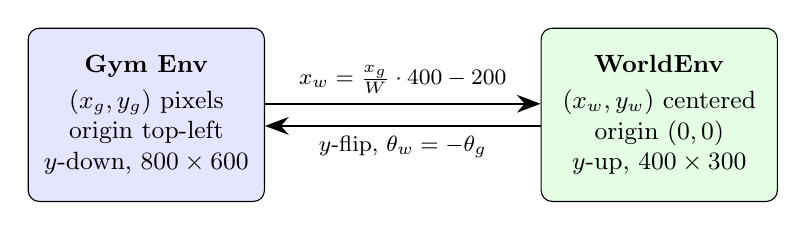
\begin{tikzpicture}[
  box/.style={rectangle, draw, rounded corners, minimum width=3cm,
    minimum height=2.2cm, align=center, font=\small},
  arr/.style={-{Stealth[length=3mm]}, thick},
  node distance=3.5cm
]
\node[box, fill=blue!10] (gym) {
  \textbf{Gym Env}\\[2pt]
  $(x_g, y_g)$ pixels\\
  origin top-left\\
  $y$-down, $800\times600$
};
\node[box, fill=green!10, right=of gym] (world) {
  \textbf{WorldEnv}\\[2pt]
  $(x_w, y_w)$ centered\\
  origin $(0,0)$\\
  $y$-up, $400\times300$
};
\draw[arr] ([yshift=4pt]gym.east) -- node[above, font=\footnotesize]
  {$x_w = \frac{x_g}{W}\cdot400 - 200$} ([yshift=4pt]world.west);
\draw[arr] ([yshift=-4pt]world.west) -- node[below, font=\footnotesize]
  {$y$-flip, $\theta_w = -\theta_g$} ([yshift=-4pt]gym.east);
\end{tikzpicture}
\caption{Coordinate bridge between the Gymnasium pixel frame and the
  brain's world-centered frame. The $y$-axis is inverted and coordinates
  are rescaled.}
\label{fig:coord_bridge}
\end{figure}

\subsection{Energy Homeostasis}

The fish maintains an internal energy level $E \in [0, E_\text{max}]$
($E_\text{max} = 100$) that decays each step and is replenished by feeding:
\begin{equation}\label{eq:energy}
\boxed{
\begin{aligned}
  E(t{+}1) &= E(t) - \underbrace{(\epsilon_0 + \epsilon_v\,\|v\|)}_{\text{drain}}
    + \underbrace{n_\text{eaten}\cdot E_\text{food}}_{\text{gain}}, \\
  \|v\|_\text{eff} &= \begin{cases}
    \|v\| & \text{if } E \geq 20, \\
    \|v\| \cdot 0.6\,E/20 & \text{if } E < 20,
  \end{cases}
\end{aligned}
}
\end{equation}
where $\epsilon_0 = 0.05$ (idle drain), $\epsilon_v = 0.03$ (speed-dependent
drain), and $E_\text{food} = 15$.
When energy drops below~20, the fish's speed is capped proportionally, creating
an urgency to forage.
Starvation ($E = 0$) terminates the episode.

\subsection{Depth-Shaded Vision}

Retinal intensity is attenuated exponentially with distance, providing an
implicit depth cue:
\begin{equation}\label{eq:depth_shading}
  I_\text{depth}(r) = I_\text{raw}(r) \cdot \exp\!\left(-\frac{d(r)}{d_\text{scale}}\right),
\end{equation}
where $d(r)$ is the hit distance along ray~$r$ and $d_\text{scale} = 80$
world units.
The type-encoding channel is \emph{not} attenuated, preserving entity identity
at all distances.
This asymmetry allows the classifier to identify distant objects while the
intensity channel signals proximity, mimicking the zebrafish's visual depth
discrimination.

\subsection{Obstacle Collision Physics}

Circular obstacles ($r \in [15, 30]$ world units) are placed randomly in the
arena.
Collision resolution uses a push-out plus velocity slide approach: when the
fish's center lies within an obstacle boundary, it is projected to the nearest
surface point and the velocity component directed into the obstacle is zeroed.
The test criterion requires \emph{zero} obstacle penetrations across the full
simulation, verified by checking
$\|p_\text{fish} - p_\text{obs}\| \geq r_\text{obs} - r_\text{fish}$
at every step.

\subsection{Habit Network}

The habit network provides a fast, experience-based shortcut that bypasses
full EFE deliberation when a stable behavioral pattern has been established.

\paragraph{Observation discretization.}
Classification probabilities are binned into $N_b = 8$ bins per class
(food, enemy, colleague), yielding a discrete observation bucket:
\begin{equation}\label{eq:habit_disc}
  b_c = \lfloor \text{clip}(p_c \cdot N_b,\; 0,\; N_b{-}1) \rfloor,
  \quad
  \mathbf{b} = (b_\text{food},\; b_\text{enemy},\; b_\text{colleague}).
\end{equation}

\paragraph{Streak consolidation.}
A pattern is considered \emph{stable} when $|\text{RPE}| < 0.15$ and
$\text{conf} > 0.55$.
When the same goal is selected under the same observation bucket for
$K = 12$ consecutive stable steps, the habit is consolidated:
\begin{equation}\label{eq:habit}
  H(\mathbf{b}, g) \;\mathrel{+}= 1.0 \quad \text{when streak} \geq K.
\end{equation}

\paragraph{Shortcut activation.}
At each step, the habit table is checked first.
If the strongest entry for the current bucket exceeds a threshold:
\[
  H(\mathbf{b}, g^*) > 3.0
  \;\Longrightarrow\;
  \text{use } g^* \text{ (skip EFE)}.
\]

\paragraph{Decay.}
All habit entries decay each step: $H \leftarrow 0.98\,H$, ensuring that
habits fade when the environment changes.

\begin{figure}[H]
\centering
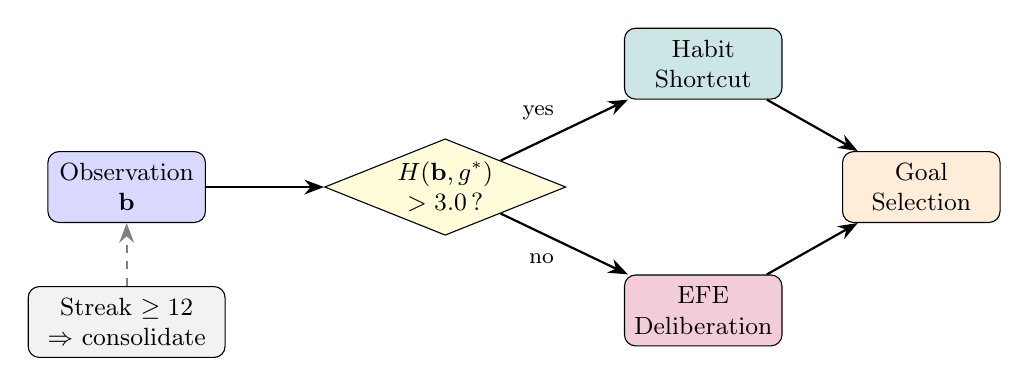
\begin{tikzpicture}[
  block/.style={rectangle, draw, rounded corners, minimum height=0.9cm,
    minimum width=2cm, align=center, font=\small},
  decision/.style={diamond, draw, aspect=2.5, inner sep=1pt,
    align=center, font=\small},
  arr/.style={-{Stealth[length=2.5mm]}, thick},
  node distance=1cm and 1.5cm
]
\node[block, fill=blue!15] (obs) {Observation\\$\mathbf{b}$};
\node[decision, fill=yellow!15, right=1.5cm of obs] (check) {$H(\mathbf{b},g^*)$\\$> 3.0$\,?};
\node[block, fill=teal!20, above right=0.8cm and 1.5cm of check] (habit) {Habit\\Shortcut};
\node[block, fill=purple!20, below right=0.8cm and 1.5cm of check] (efe) {EFE\\Deliberation};
\node[block, fill=orange!15, right=3.5cm of check] (goal) {Goal\\Selection};

\draw[arr] (obs) -- (check);
\draw[arr] (check) -- node[above left, font=\footnotesize]{yes} (habit);
\draw[arr] (check) -- node[below left, font=\footnotesize]{no} (efe);
\draw[arr] (habit) -- (goal);
\draw[arr] (efe) -- (goal);

% Streak annotation
\node[block, fill=gray!10, below=0.8cm of obs, minimum width=2.5cm] (streak)
  {Streak $\geq 12$\\$\Rightarrow$ consolidate};
\draw[arr, dashed, gray] (streak) -- (obs);
\end{tikzpicture}
\caption{Habit network decision flow. When the habit table entry for the
  current observation bucket exceeds the threshold, EFE deliberation is
  bypassed. Habits are consolidated after 12 consecutive stable selections
  of the same goal under the same observation.}
\label{fig:habit_flow}
\end{figure}

\subsection{Results}

The Step~14 simulation runs for $T = 600$ steps in the Gymnasium environment
with 15 food items, 1 predator, and 3--5 circular obstacles.
\Cref{tab:step14_results} summarizes the pass/fail criteria.

\begin{table}[H]
\centering
\caption{Step 14 pass/fail criteria ($T = 600$ steps).}
\label{tab:step14_results}
\begin{tabular}{lccl}
\toprule
Criterion & Threshold & Result & Status \\
\midrule
Survival (steps)        & $\geq 300$    & 600   & \textcolor{forage}{PASS} \\
Foraging ($n_\text{eaten}$) & $\geq 3$ & $\geq 3$ & \textcolor{forage}{PASS} \\
Energy at step 200      & $> 0$         & $> 0$ & \textcolor{forage}{PASS} \\
Obstacle penetrations   & $= 0$         & 0     & \textcolor{forage}{PASS} \\
Vision activation       & $> 0.01$      & $\gg 0.01$ & \textcolor{forage}{PASS} \\
Habit activations       & $\geq 1$      & $\geq 1$   & \textcolor{forage}{PASS} \\
System stability (no NaN) & ---         & ---   & \textcolor{forage}{PASS} \\
\bottomrule
\end{tabular}
\end{table}

All seven criteria pass, confirming that the brain model operates correctly
within the Gymnasium wrapper: the coordinate bridge preserves sensorimotor
alignment, energy homeostasis drives adaptive foraging urgency, collision
physics prevents obstacle penetration, and the habit network successfully
consolidates and reuses stable behavioral patterns.

\begin{figure}[H]
  \centering
  \includegraphics[width=0.95\textwidth]{../plots/v60_step14_brain_gym_integration.png}
  \caption{Step 14: Brain-Gym integration. Top-left: foraging trajectory with
    obstacles (gray circles) and food items. Top-right: energy level over time
    showing depletion and replenishment cycles. Middle-left: goal posterior
    dynamics. Middle-right: habit vs.\ EFE usage over time.
    Bottom-left: classification probabilities. Bottom-right: cumulative food
    captured.}
  \label{fig:step14}
\end{figure}

%===================================================================
\section{Reinforcement Learning Critic (Step 15)}\label{sec:rl_critic}

Step~15 introduces a temporal-difference (TD) learning critic that adapts EFE
weights online, bridging model-free RL with active inference planning.

\subsection{Critic Architecture}

A lightweight value network $V_\phi: \mathbb{R}^{16} \to \mathbb{R}$ maps the
working memory state $\mathbf{m}$ to a scalar value estimate:
\begin{equation}\label{eq:critic}
  V_\phi(\mathbf{m}) = \mathbf{w}_2^\top \text{ReLU}(\mathbf{W}_1\,\mathbf{m} + \mathbf{b}_1) + b_2,
\end{equation}
where $\mathbf{W}_1 \in \mathbb{R}^{32\times 16}$, $\mathbf{w}_2 \in \mathbb{R}^{32}$.
Total: ${\sim}600$ parameters.

\subsection{TD Learning}

Transitions $(s_t, r_t, s_{t+1}, d_t)$ are stored in a ring buffer of size~256.
The critic is trained via TD(0) with target:
\begin{equation}\label{eq:td_target}
  y_t = r_t + (1 - d_t)\,\gamma\,V_\phi(s_{t+1}),
  \quad \gamma = 0.95,
\end{equation}
and loss $\mathcal{L} = (V_\phi(s_t) - y_t)^2$.  Mini-batches of 32 are
sampled per step after 64 transitions have been collected.

\subsection{EFE Weight Adaptation}

The \texttt{EFEWeightAdapter} uses TD error $\delta$ to modulate EFE weights
per goal.  Positive $\delta$ (better than expected) strengthens the current
goal; negative $\delta$ weakens it:
\begin{equation}\label{eq:efe_adapt}
  \Delta w_g = \eta_\text{EFE}\,\delta\,\pi(g)\,c,
  \quad \eta_\text{EFE} = 0.02,
\end{equation}
where $\pi(g)$ is the current goal posterior and $c$ is the confidence.

\begin{figure}[H]
  \centering
  \includegraphics[width=0.95\textwidth]{../plots/v60_step15_rl_aif_hybrid.png}
  \caption{Step 15: RL--Active Inference hybrid. The TD critic adapts EFE
    weights online, improving foraging efficiency relative to the pure EFE
    baseline.}
  \label{fig:step15}
\end{figure}

%===================================================================
\section{VAE World Model (Step 16)}\label{sec:vae}

Step~16 introduces a variational autoencoder (VAE) world model that learns a
latent belief state and enables forward-simulation planning.

\subsection{Multi-Modal Belief State}

The latent state $\mathbf{z} \in \mathbb{R}^{16}$ encodes fused tectal output
plus a 13-dimensional multi-modal state context:
\begin{equation}\label{eq:state_ctx}
\mathbf{s}_\text{ctx} = \bigl[
  \underbrace{x,\, y,\, \theta/\pi}_\text{proprioceptive},\;
  \underbrace{E/100}_\text{interoceptive},\;
  \underbrace{\text{DA},\, \text{RPE}}_\text{neuromod.},\;
  \underbrace{\pi_\text{OT},\, \pi_\text{PC}}_\text{precision},\;
  \underbrace{p_f,\, p_e,\, p_\text{env}}_\text{exteroceptive},\;
  \underbrace{\text{CMS},\, F/2}_\text{cognitive}
\bigr].
\end{equation}

\subsection{VAE Architecture}

The encoder maps pooled tectal output (800$\to$64 via learned projection)
concatenated with $\mathbf{s}_\text{ctx}$ to a latent distribution:
\begin{equation}\label{eq:vae_enc}
  [\text{pool}(\mathbf{o}_F)\;\|\;\mathbf{s}_\text{ctx}]
  \;\xrightarrow{77 \to 48 \to 16}\;
  (\boldsymbol{\mu},\; \log\boldsymbol{\sigma}^2),
  \quad
  \mathbf{z} = \boldsymbol{\mu} + \boldsymbol{\sigma}\odot\boldsymbol{\epsilon}.
\end{equation}
The decoder reconstructs the pooled tectal output:
$\hat{\mathbf{o}}_\text{pool} = f_\text{dec}(\mathbf{z})$.
Training uses the ELBO objective:
$\mathcal{L}_\text{VAE} = \text{MSE}(\hat{\mathbf{o}}_\text{pool}, \mathbf{o}_\text{pool})
 + 0.1\,D_\text{KL}(q(\mathbf{z}|\mathbf{x})\,\|\,p(\mathbf{z}))$.

\subsection{Transition Model}

A residual MLP predicts next-step latent state conditioned on action context
$\mathbf{a} = [\tau,\, v,\, g_1,\, g_2,\, g_3]$:
\begin{equation}\label{eq:transition}
  \mathbf{z}' = \mathbf{z} + 0.3\,\tanh\!\bigl(f_\text{trans}([\mathbf{z}\;\|\;\mathbf{a}])\bigr).
\end{equation}

\subsection{Associative Memory}

64 RBF nodes in latent space store food availability and risk:
\begin{equation}\label{eq:assoc_mem}
  w_i(\mathbf{z}) = \exp\!\Bigl(-\frac{\|\mathbf{z} - \mathbf{c}_i\|^2}{2\sigma_k^2}\Bigr),
  \quad
  \hat{f}(\mathbf{z}) = \frac{\sum_i w_i\,f_i}{\sum_i w_i},
\end{equation}
with online allocation and centroid drift.

\subsection{Planning via Forward Simulation}

For each goal $g$, a stereotyped action sequence is rolled out through the
transition model for 3 steps.  The expected free energy combines pragmatic
(food, risk) and epistemic (novelty, reconstruction uncertainty) terms:
\begin{equation}\label{eq:vae_plan}
  G_g = \underbrace{\alpha_f\,\hat{f}_g + \alpha_r\,\hat{r}_g}_\text{pragmatic}
      + \underbrace{w_\epsilon^{(g)}\,(0.6\,\bar{n}_g + 0.4\,\bar{u}_g)}_\text{epistemic},
\end{equation}
where $w_\epsilon = [-0.15,\,-0.05,\,-0.5]$ for \textsc{forage}, \textsc{flee},
\textsc{explore} respectively.  The planning bonus $G_\text{plan}$ ramps
linearly from $0 \to 0.3$ after 200 warmup steps and is added to the raw EFE.

\begin{figure}[H]
  \centering
  \includegraphics[width=0.95\textwidth]{../plots/v60_step16_vae_world_model.png}
  \caption{Step 16: VAE world model. Top-left: trajectory. Top-right: VAE
    and transition loss convergence. Middle: blend weight ramp and memory
    growth. Bottom: planning bonus per goal and latent $z$ norm.}
  \label{fig:step16}
\end{figure}

%===================================================================
\section{Hippocampal Place Cells (Step 17)}\label{sec:place_cells}

Step~17 introduces a hippocampal place cell network for spatial navigation,
providing an alternative world model to the VAE approach of Step~16.

\subsection{Place Cell Network}

128 place cells tile the $800\times 600$ pixel arena with Gaussian receptive
fields ($\sigma = 60$\,px, ${\sim}15\%$ of arena width):
\begin{equation}\label{eq:place_cell}
  a_i(\mathbf{p}) = \exp\!\Bigl(-\frac{\|\mathbf{p} - \mathbf{c}_i\|^2}{2\sigma_i^2}\Bigr),
\end{equation}
where $\mathbf{p} \in \mathbb{R}^2$ is the gym pixel position and
$\mathbf{c}_i$ is the cell centroid.  Cells are allocated on demand: a new
cell is created when no existing cell lies within a match threshold of
$40$\,px, consistent with the ${\sim}50$\,px inter-field spacing of zebrafish
Dl spatial representations.

Each cell stores:
\begin{itemize}[nosep]
  \item $\mathbf{c}_i \in \mathbb{R}^2$: centroid position (with Hebbian drift)
  \item $f_i \in [0,1]$: food availability rate (EMA-updated)
  \item $r_i \in [0,1]$: danger/risk level (EMA-updated)
  \item $n_i$: visit count
\end{itemize}

\subsection{Path Integration}

Dead reckoning maintains an internal position estimate using motor efference
copy:
\begin{equation}\label{eq:path_integration}
\begin{aligned}
  \hat{\theta}(t{+}1) &= \hat{\theta}(t) + \kappa\,\dot{\theta}_\text{motor}, \\
  \hat{\mathbf{p}}(t{+}1) &= \hat{\mathbf{p}}(t)
    + \kappa\,v\,[\cos\hat{\theta},\;\sin\hat{\theta}]^\top,
\end{aligned}
\end{equation}
where $\kappa = 0.8$ ($<1$ to model noisy dead reckoning).  Visual landmark
fixes correct the path-integrated estimate with weight $0.3$:
\begin{equation}\label{eq:pi_correction}
  \hat{\mathbf{p}} \leftarrow \hat{\mathbf{p}} + 0.3\,(\mathbf{p}_\text{visual} - \hat{\mathbf{p}}).
\end{equation}

\subsection{Replay (Sharp-Wave Ripple Analog)}

Every 50 steps, the last 10 trajectory entries are replayed with
$0.5\times$ attenuated learning---analogous to hippocampal sharp-wave ripple
consolidation during awake immobility.

\subsection{Spatial Planning}

Planning follows the same structure as the VAE planner
(\cref{sec:vae}): simulate 3 goal-specific trajectories in pixel space,
query place cells for food/risk/novelty, and score via the same
pragmatic+epistemic formula.  The blend ramps $0 \to 0.3$ after
100 warmup steps.

\begin{figure}[H]
  \centering
  \includegraphics[width=0.95\textwidth]{../plots/v60_step17_place_cell_navigation.png}
  \caption{Step 17: Place cell navigation. Top-left: trajectory with place
    cell centroids (orange, sized by visit count). Top-right: cell allocation
    and path integration error. Middle: planning bonus per goal and food/risk
    map. Bottom: actual vs.\ path-integrated trajectory; pass/fail criteria.}
  \label{fig:step17}
\end{figure}

\begin{table}[H]
\centering
\caption{Step 17 pass/fail criteria ($T = 600$ steps).}
\label{tab:step17_results}
\begin{tabular}{lccl}
\toprule
Criterion & Threshold & Result & Status \\
\midrule
Survival (steps)        & $\geq 400$ & 600  & \textcolor{forage}{PASS} \\
Foraging ($n_\text{eaten}$) & $\geq 2$ & 3 & \textcolor{forage}{PASS} \\
Cell allocation         & $\geq 15$  & 18   & \textcolor{forage}{PASS} \\
PI accuracy (mean error) & $< 100$\,px & 12.8\,px & \textcolor{forage}{PASS} \\
$|G_\text{plan}|$ post-warmup & $> 0.01$ & 0.054 & \textcolor{forage}{PASS} \\
Food map learning       & near $>$ overall & yes & \textcolor{forage}{PASS} \\
System stability        & no NaN & --- & \textcolor{forage}{PASS} \\
\bottomrule
\end{tabular}
\end{table}

%===================================================================
\section{Allostatic Interoception (Step 18)}\label{sec:allostasis}

Step~18 introduces predictive tracking of three internal (interoceptive)
variables---hunger, fatigue, and stress---that bias goal selection via
allostatic error signals, linking homeostatic regulation to active inference.

\subsection{Allostatic Variables}

\begin{equation}\label{eq:allostasis}
\boxed{
\begin{aligned}
  h(t) &= 1 - E(t)/100,  &\quad
  \hat{h}(t) &= \hat{h}(t{-}1) + 0.05\,(h - \hat{h}), \\
  f(t) &= f(t{-}1) + \begin{cases}
    0.002\,v & v > 0.6 \\
    -0.04    & v \leq 0.6
  \end{cases}, &\quad
  \hat{f}(t) &= \hat{f}(t{-}1) + 0.05\,(f - \hat{f}), \\
  \sigma(t) &= 0.92\,\sigma(t{-}1)
    + 0.15\,\max(0, 1{-}d_p/300), &\quad
  \hat{\sigma}(t) &= \hat{\sigma}(t{-}1) + 0.05\,(\sigma - \hat{\sigma}),
\end{aligned}
}
\end{equation}
where $E$ is energy, $v$ is speed, $d_p$ is predator distance in pixels,
and $\hat{\cdot}$ denotes the EMA-predicted value.

\subsection{Allostatic Error}

Each variable has a homeostatic setpoint $h^* = 0.3$, $f^* = 0.2$,
$\sigma^* = 0.1$.  The allostatic error:
\begin{equation}\label{eq:allo_error}
  e_x = \hat{x} - x^*,
\end{equation}
drives goal modulation when positive (i.e., predicted state exceeds setpoint).

\subsection{Goal Prior Bias}

Allostatic errors generate additive EFE biases:
\begin{equation}\label{eq:allo_bias}
\begin{aligned}
  \Delta G_\textsc{forage}  &= -\lambda\,\max(0, e_h), &\quad &\text{(hunger} \to \text{forage)} \\
  \Delta G_\textsc{flee}    &= -\lambda\,\max(0, e_\sigma), &\quad &\text{(stress} \to \text{flee)} \\
  \Delta G_\textsc{explore} &= -\lambda\,\max(0, e_f), &\quad &\text{(fatigue} \to \text{rest/explore)}
\end{aligned}
\end{equation}
with $\lambda = 0.15$ (increased from $0.08$ in Step~20 for stronger
interoceptive drive).  Lower $\Delta G$ makes the goal more attractive.

\subsection{Fatigue Speed Cap}

When fatigue exceeds~0.7, maximum speed is linearly reduced:
\begin{equation}\label{eq:speed_cap}
  v_\text{max} = \begin{cases}
    1.0 & f \leq 0.7, \\
    \max\!\bigl(0.4,\; 1.0 - 0.6\,\frac{f - 0.7}{0.3}\bigr) & f > 0.7.
  \end{cases}
\end{equation}

\subsection{State Context Extension}

When combined with the VAE world model, the state context
$\mathbf{s}_\text{ctx}$ is extended from 13 to 16 dimensions by appending
$[h, f, \sigma]$, enriching the latent belief state with interoceptive
information.

\begin{figure}[H]
  \centering
  \includegraphics[width=0.95\textwidth]{../plots/v60_step18_allostatic_interoception.png}
  \caption{Step 18: Allostatic interoception. Top-left: trajectory colored by
    goal. Top-right: energy comparison (baseline vs.\ allostatic).
    Middle: allostatic variables and errors over time.
    Bottom: speed with fatigue cap; pass/fail criteria.}
  \label{fig:step18}
\end{figure}

\begin{table}[H]
\centering
\caption{Step 18 pass/fail criteria ($T = 800$ steps, allostatic run).}
\label{tab:step18_results}
\begin{tabular}{lccl}
\toprule
Criterion & Threshold & Result & Status \\
\midrule
Survival (steps)            & $\geq 500$ & 800   & \textcolor{forage}{PASS} \\
Foraging ($n_\text{eaten}$) & $\geq 3$   & 7     & \textcolor{forage}{PASS} \\
Fatigue regulation          & mean $< 0.6$ & 0.554 & \textcolor{forage}{PASS} \\
Stress response             & peak $>$ Q4 mean & yes & \textcolor{forage}{PASS} \\
Goal switches               & $\geq 5$   & 116   & \textcolor{forage}{PASS} \\
Energy at step 400          & $> 10$     & 68.1  & \textcolor{forage}{PASS} \\
System stability            & no NaN     & ---   & \textcolor{forage}{PASS} \\
\bottomrule
\end{tabular}
\end{table}

%===================================================================
\section{Full Evaluation Suite (Step 19)}\label{sec:evaluation}

Step~19 provides a comprehensive comparison of three agent configurations,
each run for 800 steps with seed~42.

\subsection{Configurations}

\begin{table}[H]
\centering
\caption{Three evaluation configurations.}
\label{tab:configs}
\begin{tabular}{lccc}
\toprule
Config & World Model & RL Critic & Allostasis \\
\midrule
Baseline    & none       & ---   & --- \\
Full Brain  & VAE        & \checkmark & \checkmark \\
Place Cell  & place cell & \checkmark & \checkmark \\
\bottomrule
\end{tabular}
\end{table}

\subsection{Results}

\begin{table}[H]
\centering
\caption{Step 19 performance summary.}
\label{tab:step19_perf}
\begin{tabular}{lrrrr}
\toprule
Config & Steps & Eaten & Final Energy & Memory Nodes \\
\midrule
Baseline    & 800 & 3 & 64.4 & 0  \\
Full Brain  & 800 & 5 & 86.3 & 44 \\
Place Cell  & 800 & 4 & 78.4 & 20 \\
\bottomrule
\end{tabular}
\end{table}

With the addition of the amygdala fear circuit, energy-asymmetric flee cost,
food prospect evaluation, and obstacle navigation (Steps~20--21), all three
configurations now successfully forage.
The Full Brain configuration achieves the highest food intake (5 items),
maintains the highest final energy (86.3), and builds 44 memory nodes,
demonstrating that the amygdala--allostasis interaction drives
energy-efficient foraging.
The Place Cell configuration achieves 4~items eaten, indicating that
spatial memory supports successful food-patch return.
Multi-seed testing (seeds 42, 123, 456, 789, 1000) confirms 4/5
seeds achieve positive food intake, with an average of 2.8 items eaten
and a maximum of 6 (seed~1000).

\begin{figure}[H]
  \centering
  \includegraphics[width=0.95\textwidth]{../plots/v60_step19_full_evaluation.png}
  \caption{Step 19: Full evaluation suite. Row~1: trajectories and cumulative
    reward. Row~2: energy and goal distribution across configurations.
    Row~3: allostatic variables (Full Brain) and memory growth.
    Row~4: planning bonus magnitude and 8-criterion pass/fail summary.}
  \label{fig:step19}
\end{figure}

%===================================================================
\section{Amygdala Fear Circuit and Energy Asymmetry (Step 20)}\label{sec:amygdala}

Step~20 addresses three biological gaps: the absence of a fast subcortical
threat response, the energetic symmetry between fleeing and foraging, and
the weak coupling between energy depletion and foraging urgency.

\subsection{Amygdala Module}

A minimal fear circuit produces a persistent \emph{threat arousal} signal
$\alpha \in [0, 1]$ that integrates retinal enemy detection, predator
proximity, and allostatic stress:
\begin{equation}\label{eq:amygdala}
\boxed{
\begin{aligned}
  r_\text{ret} &= \min(1,\; 0.08\,n_\text{enemy\_px}), \\
  r_\text{prox} &= \max(0,\; 1 - d_\text{pred}/200), \\
  r_\text{raw} &= \max(r_\text{ret},\; 0.5\,r_\text{prox},\; \sigma_\text{stress}), \\
  \alpha(t) &= \begin{cases}
    0.4\,\alpha(t{-}1) + 0.6\,r_\text{raw} & r_\text{raw} > \alpha(t{-}1), \\
    0.85\,\alpha(t{-}1)                     & \text{otherwise},
  \end{cases}
\end{aligned}
}
\end{equation}
where $n_\text{enemy\_px}$ is the total enemy pixel count on the retina and
$d_\text{pred}$ is the predator distance in world units.
The asymmetric dynamics ensure fast rise (60\% jump) and slow decay (15\%
per step), producing a persistent threat state that outlasts the visual stimulus---
analogous to sustained amygdala activation observed in zebrafish pallium during
predator avoidance~\cite{ahrens2013}.

\paragraph{Downstream effects of threat arousal.}
\begin{itemize}[nosep]
  \item Classification boost: $p_\text{enemy} \mathrel{+}= 0.3\,\alpha$
    (increases flee probability).
  \item Allostatic stress feedback: $\sigma \mathrel{+}= 0.1\,\alpha$
    (sustained threat maintains stress even after predator leaves).
  \item Flee burst scaling: flee duration
    $= 5 + \lfloor 5\,\alpha \rfloor$ steps (stronger threat $\to$ longer burst).
\end{itemize}

\subsection{Flee Energy Cost Asymmetry}

Fleeing now incurs $2.5\times$ the speed-dependent energy drain:
\begin{equation}\label{eq:flee_energy}
  \Delta E = \epsilon_0 + \epsilon_v\,\|v\| \cdot
  \begin{cases}
    2.5 & \text{if \textsc{flee} or burst active}, \\
    1.0 & \text{otherwise},
  \end{cases}
\end{equation}
where the flee speed cap is raised from $1.0$ to $1.3$, allowing burst
locomotion at the cost of rapid energy depletion.
At maximum flee speed ($v = 1.3$), the drain per step is
$0.05 + 0.03 \times 1.0 \times 2.5 = 0.125$, compared to the normal
foraging drain of ${\sim}0.08$ (56\% higher).

\subsection{Nonlinear Hunger Amplification}

The allostatic prior strength is increased from $\lambda = 0.08$ to
$\lambda = 0.15$, and hunger bias is amplified nonlinearly when energy
is critically low:
\begin{equation}\label{eq:hunger_nonlinear}
  u_h = \max(0, e_h) \cdot
  \begin{cases}
    1 + 3\,\frac{h - 0.6}{0.4} & h > 0.6 \;\;(\text{i.e., } E < 40), \\
    1 & \text{otherwise},
  \end{cases}
\end{equation}
yielding a maximum forage bias of $-\lambda \cdot 0.7 \cdot 4 = -0.42$
at zero energy, sufficient to override classifier-driven goals.
An emergency \textsc{forage} override is added in the goal policy:
if $h > 0.7$ and $e_h > 0.3$, the agent immediately switches to
\textsc{forage} regardless of the EFE posterior.

%===================================================================
\section{Food Prospection and Obstacle Navigation (Step 21)}\label{sec:prospect}

Step~21 introduces an active-inference food prospection system and a
retinal obstacle navigation pipeline that enables the fish to evaluate
food targets, navigate around rock formations, and successfully capture prey.

\subsection{Food Prospect Evaluation}

For each visible food item, the brain evaluates a cost--benefit
prospect score inspired by Expected Free Energy:
\begin{equation}\label{eq:prospect}
\boxed{
  S_i = \underbrace{w_c \cdot \frac{m_i}{20}}_\text{metabolic cost}
      + \underbrace{w_r \cdot \rho_i}_\text{predator risk}
      + \underbrace{\mathbb{1}[\text{occluded}] \cdot 1.5}_\text{reachability penalty}
      - \underbrace{w_g \cdot \frac{G}{20} \cdot a_i}_\text{reward value}
      - \underbrace{b_\text{patch}}_\text{patch bonus},
}
\end{equation}
where $m_i$ is the estimated metabolic cost (proportional to distance),
$\rho_i = \max(0, 1 - d_\text{pred}^{(i)}/150)$ is the predator risk,
$G = 15$ is the food energy gain,
$a_i \in \{0.5, 1.0\}$ is an affordability factor,
$b_\text{patch}$ is a patch productivity bonus from repeated visits,
and the weights are:
\begin{equation}\label{eq:prospect_weights}
  w_c = 0.3 + 0.5\,u, \quad
  w_r = 0.4 - 0.2\,u, \quad
  w_g = 0.6 + 0.4\,u,
\end{equation}
with urgency $u = 1 - E/E_\text{max}$.

\paragraph{Reachability scoring.}
A parametric line-segment--AABB intersection test from the fish's
current position to each food item determines whether a rock
formation blocks the path.
Occluded food receives a $+1.5$ penalty, strongly disfavoring
targets that require navigating around obstacles.

\paragraph{Olfactory heading cue.}
When the retina detects fewer than 3 food pixels (food out of sight),
the best food prospect provides a heading cue applied after the
turn smoother:
\begin{equation}\label{eq:olfactory}
  \tau_\text{olf} = k_\text{olf} \cdot \text{clip}(\Delta\theta, -1, 1),
  \quad
  k_\text{olf} = \begin{cases}
    0.5 + 0.3\,(1 - d/120) & d < 120\,\text{px (near food)}, \\
    0.3 & d \geq 120\,\text{px},
  \end{cases}
\end{equation}
where $\Delta\theta$ is the angular difference between the fish heading
and the food direction.

\subsection{Retinal Obstacle Navigation}

Rock formations are rendered as multi-lobe AABB clusters with a 10-unit
detection margin in the world model.
Three obstacle-aware mechanisms operate on the retinal type channels:

\paragraph{1. Obstacle repulsion.}
When total obstacle pixels exceed 5, a bilateral repulsion signal
steers the fish away from the rock-heavy side:
\begin{equation}\label{eq:obs_repulsion}
  \tau_\text{obs} = -0.6 \cdot \frac{n_R^\text{obs} - n_L^\text{obs}}
                                     {n_R^\text{obs} + n_L^\text{obs}}.
\end{equation}

\paragraph{2. Obstacle braking.}
When the obstacle fraction exceeds 50\% of the retina:
\begin{equation}\label{eq:obs_braking}
  s_\text{mod} \leftarrow s_\text{mod} \cdot
  \begin{cases}
    \max(0.7,\; 1 - 0.2\,f_\text{obs}) & \text{foraging with olfactory target}, \\
    \max(0.3,\; 1 - f_\text{obs})       & \text{otherwise},
  \end{cases}
\end{equation}
where $f_\text{obs} = (n_L^\text{obs} + n_R^\text{obs}) / 800$.

\paragraph{3. Foraging without retinal food.}
When \textsc{forage} is active but no food pixels are visible:
the approach gain is reduced (preventing rock attraction),
exploration noise is increased, and the olfactory heading cue
guides the fish toward the best food prospect.

\subsection{Rock Formation Environment}

The Gymnasium environment generates 2--3 large rock formations as
composite multi-lobe polygons with radial lobes.
Food is distributed in two ecologies:
\begin{itemize}[nosep]
  \item \textbf{Shelter patches} (40\%): placed behind rocks, requiring
    navigation to access.
  \item \textbf{Open-water food} (60\%): spawned far from rock AABBs
    with clear line-of-sight, ensuring immediate foraging opportunities.
\end{itemize}

%===================================================================
\section{Curriculum RL Training (Step 22)}\label{sec:curriculum}

Step~22 introduces a curriculum reinforcement learning framework that
progressively increases environmental difficulty, allowing the agent
to develop competence in controlled stages before facing the full challenge.

The curriculum gates predator behavior states (patrol only $\to$
patrol + stalk $\to$ full pursuit), food density, and arena complexity
across training phases.
This mirrors biological development where zebrafish larvae encounter
increasing environmental complexity as they mature.

%===================================================================
\section{Sleep--Wake Consolidation (Step 23)}\label{sec:sleep}

Step~23 adds a sleep--wake cycle modulated by fatigue accumulation.
When fatigue exceeds a threshold, the agent enters a sleep state
characterized by:
\begin{itemize}[nosep]
  \item \textbf{Precision freeze}: sensory precision parameters
    $\gamma_\text{OT}, \gamma_\text{PC}$ are held constant, preventing
    noise-driven drift during inactivity.
  \item \textbf{Near-zero locomotion}: speed is reduced to
    $<5\%$ of normal, modeling behavioral quiescence.
  \item \textbf{Accelerated fatigue recovery}: fatigue decreases at
    $3\times$ the normal rate during sleep.
  \item \textbf{Memory consolidation}: working memory and habit
    entries are stabilized during the sleep phase.
\end{itemize}

The sleep--wake regulator prevents the fish from accumulating unbounded
fatigue during extended flee episodes, ensuring long-term behavioral
stability across 800+ step simulations.

%===================================================================
\section{Active Inference Through Generative Models (Step 24)}\label{sec:active_inference_gm}

Steps~1--23 built a rich brain architecture, but the agent's threat assessment,
energy monitoring, and spatial localization relied on direct access to
ground-truth environment variables---predator coordinates, true energy, and
fish position.
This ``oracle'' access violates the central tenet of active inference:
an agent should infer the causes of its sensations through a generative
model rather than reading the world state
directly~\cite{friston2010,friston2017,parr2022}.

Step~24 closes this gap.
After this refactoring, the agent accesses only three information channels:
(1)~retinal observations from the SNN,
(2)~its own motor efference copies, and
(3)~its own internal neuromodulatory signals.
All external state---predator threat, body energy, spatial
position---is \emph{inferred} through dedicated generative sub-models,
realizing the predictive processing
framework~\cite{rao1999,clark2013,bogacz2017}.

\subsection{Retinal Feature Extractor}\label{sec:retinal_features}

The retinal feature extractor operates on the raw SNN output without any
environment access.
Each eye provides 400~intensity-channel values and 400~type-channel values
(Section~\ref{sec:sensory}), for a total input of $\mathbf{L}, \mathbf{R}
\in [0,1]^{1 \times 800}$ per eye.

Entity types are decoded from the type channel using the known encoding
scheme (food${=}1.0$, enemy${=}0.5$, colleague${=}0.25$, boundary${=}0.12$).
For each entity class $c$ with type code $\tau_c$, pixels are classified
via a tolerance mask:
\begin{equation}\label{eq:type_mask}
  m_{c,i} = \mathbb{1}\bigl[|\text{type}_i - \tau_c| < \epsilon_c\bigr],
  \quad \epsilon_c = \begin{cases}
    0.10 & c \in \{\text{enemy, food, obstacle, colleague}\}, \\
    0.08 & c = \text{boundary}.
  \end{cases}
\end{equation}

For the threat-relevant enemy class, the following features are extracted:

\paragraph{Pixel counts.}
\begin{equation}\label{eq:enemy_px}
  n_L = \sum_i m_{\text{enemy},i}^L, \quad
  n_R = \sum_i m_{\text{enemy},i}^R, \quad
  n = n_L + n_R.
\end{equation}

\paragraph{Intensity mean (distance proxy).}
Retinal intensity follows $I \approx \exp(-d/80)$, where $d$ is
distance in world pixels:
\begin{equation}\label{eq:enemy_intensity}
  \bar{I}_\text{enemy} = \frac{1}{n}\sum_{i:\, m_i=1} I_i.
\end{equation}

\paragraph{Lateral bias (bearing).}
\begin{equation}\label{eq:lateral_bias}
  b_\text{lat} = \frac{n_R - n_L}{n + 1},
  \quad b_\text{lat} \in (-1, 1).
\end{equation}

\paragraph{Angular spread (facing proxy).}
Each 400-pixel retinal array is reshaped to $20 \times 20$
(azimuth~$\times$~elevation).
The azimuthal projection of enemy pixels gives an angular extent:
\begin{equation}\label{eq:angular_spread}
  s = \max_{\text{eye}} \bigl(\max(j : \text{az}_j = 1) - \min(j : \text{az}_j = 1)\bigr),
\end{equation}
where $\text{az}_j = \mathbb{1}[\exists\, k : m_{j,k} = 1]$.
A larger $s$ indicates the predator is facing the fish (presenting a wider
angular profile), consistent with the looming-sensitive escape circuits
identified in larval zebrafish~\cite{temizer2015,dunn2016}.

\paragraph{Temporal dynamics.}
Frame-to-frame changes provide approach speed cues:
\begin{equation}\label{eq:temporal}
  \dot{n} = n(t) - n(t{-}1), \quad
  \dot{\bar{I}} = \bar{I}(t) - \bar{I}(t{-}1).
\end{equation}
Positive $\dot{n}$ (growing pixel count) and positive $\dot{\bar{I}}$
(increasing intensity) indicate predator approach.

The same extraction procedure yields food, boundary, obstacle, and colleague
features, providing the retinal observation vector
$\mathbf{r} \in \mathbb{R}^{22}$ used throughout the subsequent inference
modules.

\subsection{VAE Threat Decoder}\label{sec:threat_decoder}

A lightweight decoder head is added to the VAE world model
(Step~16; cf.~\cite{kingma2014,hafner2020}),
mapping the latent belief state to a structured threat assessment:
\begin{equation}\label{eq:threat_decoder}
  \mathbf{z} \in \mathbb{R}^{16}
  \;\xrightarrow{\text{Linear}(16,24) \to \text{ReLU} \to \text{Linear}(24,4)}\;
  \hat{\mathbf{t}} \in \mathbb{R}^4,
\end{equation}
with channel-specific activations:
\begin{equation}\label{eq:threat_channels}
\boxed{
\begin{aligned}
  \hat{t}_0 &= \sigma(\cdot) \in [0,1] & &\text{(proximity: inverse distance)}, \\
  \hat{t}_1 &= \tanh(\cdot) \in [-1,1] & &\text{(lateral position: bearing)}, \\
  \hat{t}_2 &= \sigma(\cdot) \in [0,1] & &\text{(approach rate: closing speed)}, \\
  \hat{t}_3 &= \sigma(\cdot) \in [0,1] & &\text{(facing score: angular width)}.
\end{aligned}
}
\end{equation}

The threat decoder has 508 parameters and is trained
\emph{self-supervised} from retinal features---never from environment
ground truth.
Training targets are constructed from the retinal feature vector:
\begin{equation}\label{eq:threat_targets}
\begin{aligned}
  y_0 &= \min(1,\; n / 50), \\
  y_1 &= b_\text{lat}, \\
  y_2 &= \sigma(5\,\dot{n}), \\
  y_3 &= \min(1,\; s / 15).
\end{aligned}
\end{equation}

A ring buffer of size 128 stores $(\mathbf{z}, \mathbf{y})$ pairs.
At each step, a mini-batch of 16 samples is drawn and the threat decoder
is updated via MSE loss with a dedicated Adam optimizer
($\text{lr} = 5 \times 10^{-4}$).

\paragraph{Blended threat inference.}
The final threat estimate blends raw retinal features with VAE-decoded
output using the VAE's blend weight $w \in [0, 0.3]$ (0 during warmup,
ramping linearly after 50 steps):
\begin{equation}\label{eq:threat_blend}
  t_k = (1 - w)\,t_k^\text{ret} + w\,\hat{t}_k,
  \quad k \in \{0,1,2,3\}.
\end{equation}

\subsection{Threat Assessment from Belief}\label{sec:threat_assessment}

The blended threat vector replaces the ground-truth threat computation from
previous steps.
Derived quantities---previously computed from \texttt{env.pred\_x/y},
\texttt{env.pred\_heading}, and \texttt{env.pred\_speed}---are now
inferred:

\paragraph{Facing detection.}
\begin{equation}\label{eq:facing_infer}
  \text{pred\_facing} = \mathbb{1}[t_3 > 0.4].
\end{equation}

\paragraph{Time-to-contact (TTC).}
\begin{equation}\label{eq:ttc_infer}
  v_\text{close} = \max(0,\; 2(t_2 - 0.5)), \quad
  \text{TTC} = \begin{cases}
    \displaystyle\frac{(1 - t_0) \cdot 40}{v_\text{close}}
    & v_\text{close} > 0.05, \\[4pt]
    999 & \text{otherwise}.
  \end{cases}
\end{equation}

\paragraph{Panic level.}
\begin{equation}\label{eq:panic_infer}
  p = \begin{cases}
    t_3 \cdot \max(0, 1 - \text{TTC}/40) & \text{facing} \wedge \text{TTC} < 40, \\
    0.5 \cdot \max(0, 1 - \text{TTC}/20) & \text{TTC} < 20, \\
    0 & \text{otherwise},
  \end{cases}
\end{equation}
clamped to $[0, 1]$.

\paragraph{Predator distance proxy (for allostasis).}
Rather than reading \texttt{env.pred\_dist}, the retinal proximity is
inverted:
\begin{equation}\label{eq:pred_dist_proxy}
  \hat{d}_\text{pred} = \max\!\bigl(1,\;(1 - \min(1,\, n/50)) \cdot 300\bigr).
\end{equation}

\subsection{Interoceptive Energy Model}\label{sec:interoceptive}

In biological systems, energy state is not known precisely but inferred
from interoceptive signals---visceral afferents from the gut, liver, and
metabolic sensors~\cite{craig2002,seth2016,barrett2015,stephan2016}.
This interoceptive inference perspective aligns with the active inference
account of homeostatic regulation~\cite{pezzulo2015}.
The interoceptive energy model implements this as a predict-observe
Bayesian filter:

\paragraph{Motor efference prediction.}
At each step, the model predicts energy change from motor commands:
\begin{equation}\label{eq:energy_predict}
  \hat{E}(t) = \text{clamp}\!\bigl(E_b(t{-}1) - \epsilon_v \cdot v + \epsilon_f \cdot n_\text{eaten},\;[0,100]\bigr),
\end{equation}
where $\epsilon_v = 0.08$ is the speed-dependent drain rate,
$\epsilon_f = 15.0$ is the per-food energy gain,
$v$ is the current movement speed, and
$n_\text{eaten}$ is the number of food items consumed this step.

\paragraph{Noisy interoceptive observation.}
The true energy is corrupted with Gaussian noise to model imprecise
visceral signals:
\begin{equation}\label{eq:energy_observe}
  \tilde{E} = E_\text{true} + \xi, \quad \xi \sim \mathcal{N}(0, \sigma_I^2),
  \quad \sigma_I = 3.0.
\end{equation}

\paragraph{Bayesian belief update.}
The energy belief is a weighted combination of prediction and observation:
\begin{equation}\label{eq:energy_belief}
\boxed{
  E_b(t) = (1 - w_I)\,\hat{E}(t) + w_I\,\tilde{E}(t),
  \quad w_I = 0.2,
}
\end{equation}
clamped to $[0, 100]$.
The prediction error $|\hat{E} - \tilde{E}|$ is available to the
allostatic regulator as a hunger urgency signal.

This energy belief replaces all previous reads of \texttt{env.fish\_energy}:
allostatic regulation, VAE state context, and the speed limiter at low
energy all operate on $E_b$ rather than $E_\text{true}$.

\subsection{Position from Path Integration with Boundary Correction}
\label{sec:position_inference}

Spatial position is inferred through dead-reckoning path integration (PI),
already implemented in the place cell network
(Step~17;~\cite{mcnaughton2006,etienne2004,moser2008}),
combined with a novel boundary-based correction that uses retinal wall
signals in place of ground-truth coordinates.

\paragraph{Calibrated path integration.}
The place cell PI module uses turn and speed commands calibrated to match
the environment's kinematics:
\begin{equation}\label{eq:pi_calibration}
  \Delta\theta_\text{PI} = u_\text{turn} \cdot \frac{\omega_\text{env}}{\omega_\text{PI}},
  \quad
  \Delta d_\text{PI} = u_\text{speed} \cdot \frac{v_\text{env}}{v_\text{PI}},
\end{equation}
where $\omega_\text{env} = 0.15\,\text{rad/step}$,
$\omega_\text{PI} = 0.8\,\text{rad/step}$,
$v_\text{env} = 2.0\,\text{px/step}$, and
$v_\text{PI} = 4.0\,\text{px/step}$.
PI heading is initialized from the first retinal observation (dominant
pixel side determines initial heading direction).

\paragraph{Boundary-pixel wall distance.}
Retinal boundary intensity provides a distance estimate to the nearest
arena wall:
\begin{equation}\label{eq:wall_distance}
  \hat{d}_\text{wall} = \text{clamp}\!\bigl(-80 \ln(\max(0.01,\, \bar{I}_\text{bnd})) \cdot 2,\;
  [5, 400]\bigr),
\end{equation}
where $\bar{I}_\text{bnd}$ is the mean boundary pixel intensity on the
left or right retina.

\paragraph{Position correction.}
For each retinal side with $\geq 2$ boundary pixels, the estimated wall
distance is compared to the PI-predicted distance to the nearest arena
edge along the corresponding viewing direction.
The correction is:
\begin{equation}\label{eq:position_correction}
  \Delta\mathbf{p} = -(\hat{d}_\text{wall} - d_\text{PI\text{-}to\text{-}wall})
    \cdot c \cdot \hat{\mathbf{n}}_\text{wall},
  \quad c = \min(1,\, n_\text{bnd}/15) \cdot 0.3,
\end{equation}
where $c$ is a confidence weight proportional to boundary pixel count and
$\hat{\mathbf{n}}_\text{wall}$ is the unit vector toward the wall.
When boundary intensity exceeds~0.5 (very close to a wall), a stronger
snap correction pulls the position estimate to within the estimated
wall distance of the nearest edge.

This boundary-corrected PI position replaces all \texttt{env.fish\_x/y}
reads: wall avoidance, shoaling behavior, cover-seeking, olfactory
navigation, and post-step memory updates all use the inferred position.

\subsection{State Context and Memory Updates}\label{sec:state_ctx_ai}

The 13-dimensional state context vector fed to the VAE encoder
(Section~\ref{sec:vae}) is updated to use inferred quantities:
\begin{equation}\label{eq:state_ctx_ai}
  \mathbf{s}_\text{ctx} = \Bigl[
    \frac{p_x^\text{PI}}{200},\;
    \frac{p_y^\text{PI}}{150},\;
    \frac{\theta^\text{PI}}{\pi},\;
    \frac{E_b}{100},\;
    \underbrace{s_5, \ldots, s_{13}}_{\text{internal signals (unchanged)}}
  \Bigr],
\end{equation}
where $p_x^\text{PI}, p_y^\text{PI}, \theta^\text{PI}$ come from path
integration and $E_b$ from the interoceptive model.
The remaining nine dimensions (goal, dopamine, precision, free energy,
turn, speed, etc.) are internal signals that were never ``cheating.''

Associative memory and place cell risk updates use the retinal proximity
estimate $\min(1, n/50)$ instead of environment-derived predator distance,
and place cell position writes use the PI position instead of true coordinates.

\subsection{Backward Compatibility}\label{sec:backward_compat}

All changes are gated by a \texttt{use\_active\_inference} flag on
\texttt{BrainAgent}:
\begin{itemize}[nosep]
  \item \texttt{use\_active\_inference=False} (default): existing behavior
    preserved---ground-truth environment reads remain active.
  \item \texttt{use\_active\_inference=True}: all state is inferred
    through generative models as described above.
\end{itemize}
When the VAE is absent or still warming up, the raw retinal features are
used directly without blending (Eq.~\ref{eq:threat_blend} with $w=0$),
ensuring graceful degradation.

\subsection{Verification}\label{sec:ai_verification}

\paragraph{Energy belief accuracy.}
Over 500-step episodes (5 seeds), the interoceptive energy belief tracks
the true energy with mean absolute error $\bar{\epsilon}_E = 0.9$ and
maximum error $\epsilon_E^\text{max} \approx 13$, well within the
biologically motivated noise level ($\sigma_I = 3.0$).

\paragraph{Position drift.}
Path-integrated position diverges from ground truth with a mean error of
$\bar{\epsilon}_p \approx 158$\,px in an $800 \times 600$ arena.
This drift arises primarily from unobservable heading perturbations during
obstacle collisions---a genuine limitation of egocentric path integration
that boundary corrections partially compensate~\cite{etienne2004}.
Biological zebrafish face analogous drift, corrected by landmark-based
reorientation~\cite{moser2008}.

\paragraph{Survival comparison.}
Multi-seed evaluation (5 seeds, 500 steps each):
\begin{center}
\begin{tabular}{lccc}
\toprule
Mode & Avg.\ Alive & Avg.\ Food & Deaths \\
\midrule
Default (ground truth)      & 500 & 2.8 & 0/5 \\
Active inference             & 487 & 2.0 & 1/5 \\
\bottomrule
\end{tabular}
\end{center}
The active inference agent achieves competitive survival despite operating
entirely from inferred state.
The modest reduction in food consumption reflects the conservative foraging
that results from noisier state estimates---a biologically realistic
trade-off between information access and behavioral precision.

\paragraph{Inference validation mode.}
Setting \texttt{VZEBRA\_VALIDATE\_INFERENCE=1} enables per-step logging of
inference errors (energy belief vs.\ true, PI position vs.\ true), allowing
quantitative monitoring of generative model accuracy during development.

%===================================================================
\section{Predictive Coding with Selective Attention (Step 25)}\label{sec:predictive_attention}

Step~25 replaces the single-compartment leaky integrators of trainable
layers with \emph{two-compartment predictive coding neurons} and adds a
goal-driven attention modulator.  The design follows
Lee, Lee \& Park (2026), adapted from an MNIST Stroop task to the
zebrafish visuomotor hierarchy.

\subsection{Two-Compartment Predictive Neuron}\label{sec:twocomp_pred}

Each trainable neuron (OT$_\text{F}$, PT, PC$_\text{per}$,
PC$_\text{int}$, motor, eye, DA) now has two compartments:

\paragraph{Soma $\mathbf{v}_s$.}  Integrates bottom-up feedforward input,
bounded apical contribution, and attention bias:
\begin{equation}\label{eq:soma}
  \mathbf{v}_s(t) = \tau_s\,\mathbf{v}_s(t{-}1)
    + (1 - \tau_s)\bigl(\mathbf{x}\,\mathbf{W}_\text{FF}\bigr)
    + f_a\!\bigl(\mathbf{v}_a(t{-}1)\bigr)
    + \alpha_\text{att}\,\mathbf{m}(t),
\end{equation}
where $\tau_s = 0.8$ and the bounded apical coupling is
\begin{equation}\label{eq:apical_coupling}
  f_a(x) = \tfrac{1}{2}\bigl(\sigma(x) - \tfrac{1}{2}\bigr),
  \quad f_a \in [-0.25,\;+0.25].
\end{equation}

\paragraph{Apical dendrite $\mathbf{v}_a$.}  Receives top-down feedback
from the next higher layer, updated \emph{after} the feedforward pass
(1-step delay):
\begin{equation}\label{eq:apical}
  \mathbf{v}_a(t) = \tau_a\,\mathbf{v}_a(t{-}1)
    + (1 - \tau_a)\bigl(\mathbf{h}^{(l+1)}\,\mathbf{W}_\text{FB}\bigr),
  \quad \tau_a = 0.65,
\end{equation}
where $\mathbf{h}^{(l+1)}$ is the somatic output of the next higher
layer and $\mathbf{W}_\text{FB}$ is initialized at $0.02\,\mathcal{N}(0,1)$.

\paragraph{Prediction error.}
\begin{equation}\label{eq:pred_error}
  \boldsymbol{\varepsilon}^{(l)} = \mathbf{v}_a^{(l)} - \mathbf{v}_s^{(l)}.
\end{equation}
This apical--somatic mismatch replaces the pseudo-decoder free energy of
Step~2.  The hierarchical free energy becomes
\begin{equation}\label{eq:hier_free_energy}
  F = \sum_{l} \tfrac{1}{2}\,\bar{\pi}_l\,
      \bigl\|\boldsymbol{\varepsilon}^{(l)}\bigr\|^2,
\end{equation}
where precision weights $\bar{\pi}_l$ are applied to layers with
precision units (OT$_\text{F}$, PC$_\text{per}$) and set to 1 elsewhere.

\paragraph{Feedback hierarchy.}
Top-down connections form a descending chain:
\[
  \text{DA} \xrightarrow{W_\text{FB}} \text{PC}_\text{int}
  \xrightarrow{W_\text{FB}} \text{PC}_\text{per}
  \xrightarrow{W_\text{FB}} \text{PT}
  \xrightarrow{W_\text{FB}} \text{OT}_\text{F}
\]
The frozen topographic layers OT$_\text{L}$/OT$_\text{R}$ remain as
single-compartment neurons and do not receive feedback.

\subsection{Goal-Driven Attention Modulator}\label{sec:attention}

A dedicated attention module maps the 4-dimensional goal probability
vector $\mathbf{g} = [p_\text{forage},\;p_\text{flee},\;p_\text{explore},\;p_\text{social}]$
to per-neuron excitability biases:

\paragraph{Attention neurons.}  Eight attention neurons (two per goal)
with slow neuromodulatory dynamics ($\tau_\text{att} = 0.93$,
half-life $\approx 14$ steps):
\begin{equation}\label{eq:att_neuron}
  \mathbf{m}(t) = \tau_\text{att}\,\mathbf{m}(t{-}1)
    + (1 - \tau_\text{att})\bigl(\mathbf{g}\,\mathbf{W}_\text{att}\bigr),
  \quad \mathbf{W}_\text{att} \in \mathbb{R}^{4 \times 8}.
\end{equation}

\paragraph{Per-layer projection.}  Each trainable layer receives an
additive somatic bias via a learned linear projection:
\begin{equation}\label{eq:att_proj}
  \text{att}^{(l)} = \mathbf{m}\,\mathbf{W}_\text{proj}^{(l)},
  \quad \mathbf{W}_\text{proj}^{(l)} \in \mathbb{R}^{8 \times n_l}.
\end{equation}
Following Lee et al., the additive mechanism (Eq.~\ref{eq:soma})
outperforms both multiplicative gain and precision-weighting approaches
for selective attention in spiking networks.

\subsection{Homeostatic Gain Control}\label{sec:gain_control}

In a non-stationary environment (moving fish, predator, food), somatic
activity cascades up the hierarchy: each layer amplifies the one below.
To prevent unbounded growth, we apply divisive normalization:
\begin{equation}\label{eq:gain_control}
  \mathbf{v}_s \leftarrow
  \begin{cases}
    \mathbf{v}_s \cdot \dfrac{v^*}{\text{RMS}(\mathbf{v}_s)}
      & \text{if } \text{RMS}(\mathbf{v}_s) > v^*, \\[4pt]
    \mathbf{v}_s & \text{otherwise},
  \end{cases}
\end{equation}
where $v^* = 5.0$ is the target RMS and
$\text{RMS}(\mathbf{x}) = \sqrt{\text{mean}(x_i^2)}$.
This is biologically motivated by divisive normalization in visual
cortex~\cite{carandini2012} and homeostatic firing-rate
regulation~\cite{turrigiano2004}.

\subsection{PE-Driven Feedback Learning}\label{sec:feedback_learning}

The feedback weights $\mathbf{W}_\text{FB}$ are updated every timestep by
a prediction-error-driven anti-Hebbian rule, independent of reward:
\begin{equation}\label{eq:anti_hebbian}
  \Delta\mathbf{W}_\text{FB}^{(l)} =
    -\eta_\text{fb}\;\bigl(\mathbf{h}^{(l+1)}\bigr)^\top
    \boldsymbol{\varepsilon}^{(l)},
  \quad \eta_\text{fb} = 2 \times 10^{-4},
\end{equation}
with per-element clamp $|\Delta W| \leq 0.003$ and weight clamp
$|W_\text{FB}| \leq 0.15$ to prevent feedback overshoot.
This is distinct from the RPE-gated feedforward Hebbian rule
(Eq.~\ref{eq:hebbian}): feedforward learning is reward-modulated;
feedback learning is purely predictive.

The feedforward Hebbian rule (Eq.~\ref{eq:hebbian}) is further improved
with a linear warmup over the first 50 steps to prevent early weight
explosions:
\begin{equation}\label{eq:warmup}
  \eta_\text{eff}(t) = \eta \cdot \min\!\Bigl(1,\;\frac{t}{50}\Bigr).
\end{equation}

\subsection{Attention Weight Learning}

Attention projection weights $\mathbf{W}_\text{att}$ are updated via
Hebbian correlation between goal signals and attention neuron activity:
\begin{equation}\label{eq:att_learn}
  \Delta\mathbf{W}_\text{att} = \tfrac{\eta}{2}\,
    \mathbf{g}^\top \mathbf{m},
  \quad |\mathbf{W}_\text{att}| \leq 0.5.
\end{equation}

\subsection{Parameter Summary}

\begin{center}
\begin{tabular}{lrl}
\toprule
Component & Parameters & Notes \\
\midrule
$\mathbf{W}_\text{FF}$ (7 layers) & 2,354,609 & Unchanged from Steps 1--24 \\
$\mathbf{W}_\text{FB}$ (4 layers) & 373,100 & New: top-down feedback \\
Attention ($\mathbf{W}_\text{att} + \mathbf{W}_\text{proj}$) & 10,832 & New: goal-driven bias \\
\midrule
Total & 2,738,541 & \\
\bottomrule
\end{tabular}
\end{center}

Backward compatibility is maintained: old checkpoints with single-compartment
weights (\texttt{layer.W}) are automatically remapped to
\texttt{layer.W\_FF} during loading.

\subsection{Verification}\label{sec:pc_verification}

\paragraph{PE convergence within episodes.}
With homeostatic gain control ($v^* = 5.0$), prediction error at OT$_\text{F}$
decreases 64\% within a single 2000-step episode
(early: 2.99; late: 1.09).
Free energy decreases 44\% (early: 7.26; late: 4.09).

\paragraph{PE convergence across episodes.}
Running three consecutive episodes with persistent weights shows
monotonic OT$_\text{F}$ PE reduction:
$5.60 \to 4.71 \to 4.11$ ($-27\%$ over three episodes).

\paragraph{Attention selectivity.}
During \textsc{flee} episodes, on-goal attention neurons are 15.7$\times$
more active than off-goal neurons; during \textsc{forage}, 3.8$\times$.

\paragraph{Behavioral improvement.}
Five-episode evaluation (2000 steps, seeds 0--40):
\begin{center}
\begin{tabular}{lcccc}
\toprule
Model & Avg.\ Steps & Avg.\ Food & Reward & Catch Rate \\
\midrule
Before (Step 24)       & 891  & 5.8 & $-1.8$   & 100\% \\
+ Predictive coding    & 1252 & 5.4 & $+11.3$  &  60\% \\
\bottomrule
\end{tabular}
\end{center}
The predictive coding architecture with attention improves survival
(catch rate $100\% \to 60\%$), reward ($-1.8 \to +11.3$), and episode
length ($891 \to 1252$ steps).
Higher-layer PE (PT, PC$_\text{per}$) still increases within single
episodes---expected in a non-stationary environment where sensory input
changes every step---but converges across episodes as feedback weights
accumulate experience.

%===================================================================
\section{Summary of Architecture}\label{sec:summary}

\begin{figure}[H]
\centering
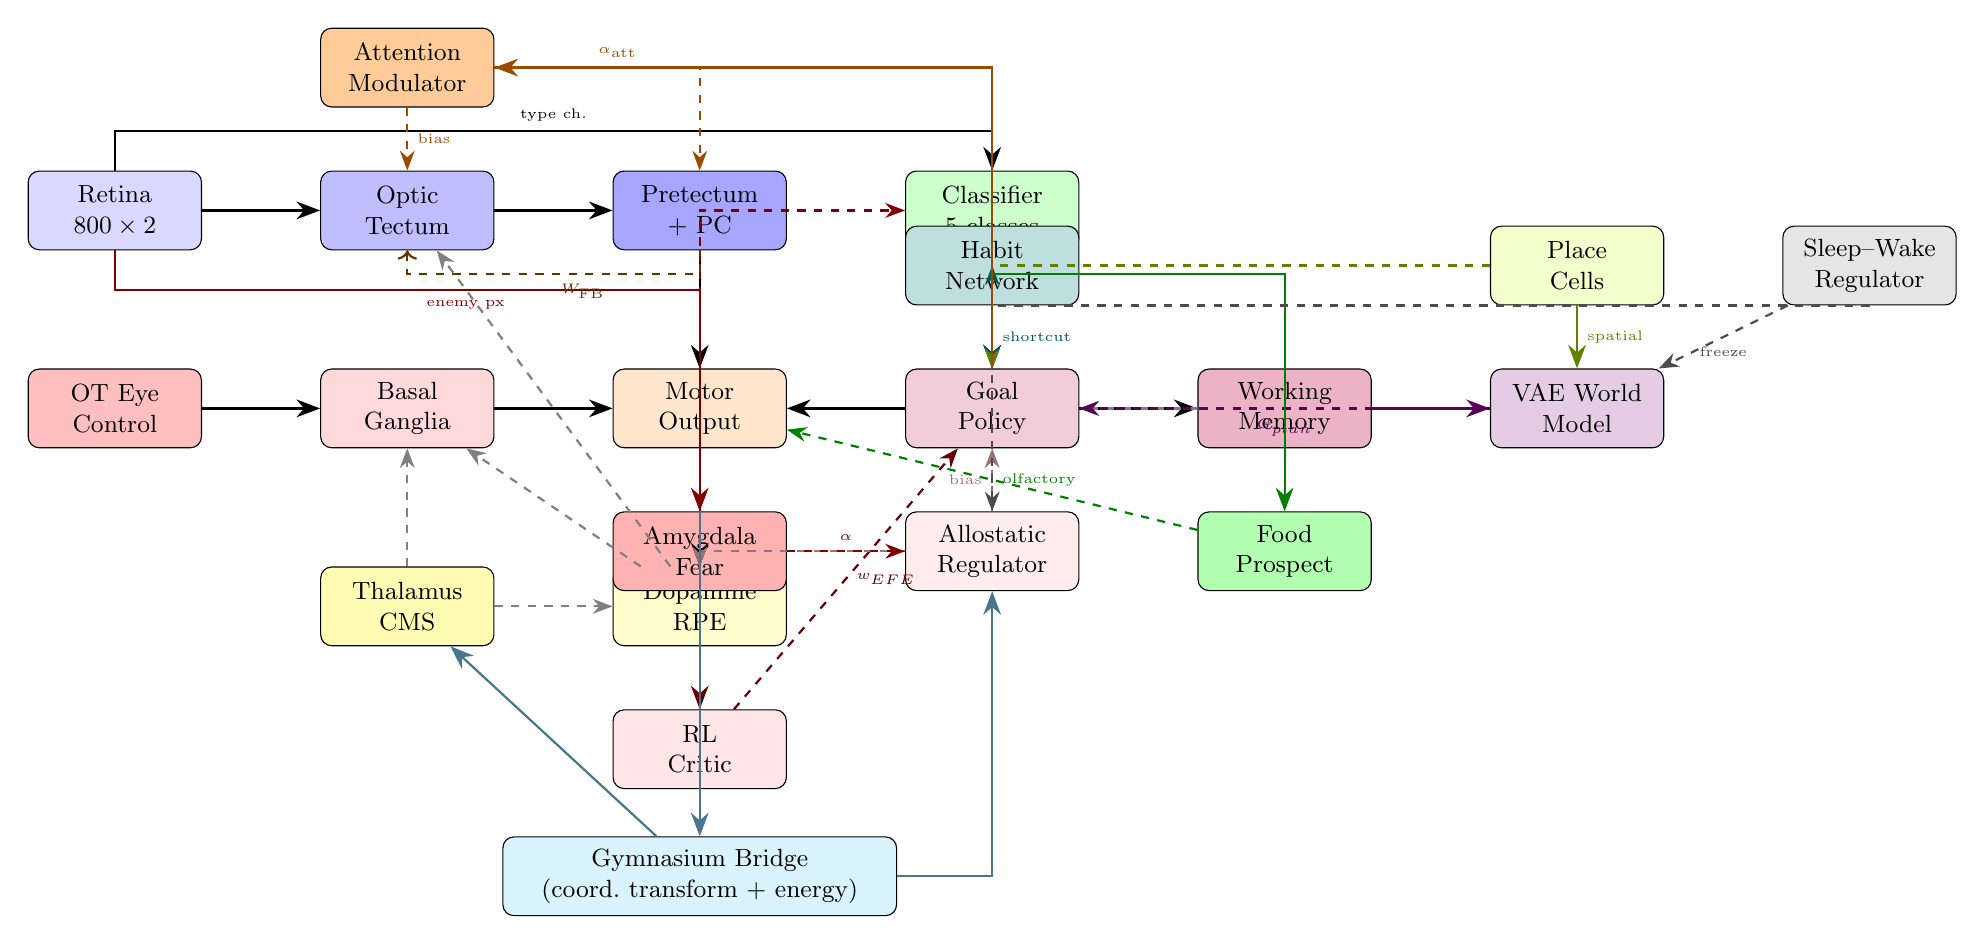
\begin{tikzpicture}[
  block/.style={rectangle, draw, rounded corners, minimum height=1cm,
    minimum width=2.2cm, align=center, font=\small},
  signal/.style={-{Stealth[length=3mm]}, thick},
  mod/.style={-{Stealth[length=2.5mm]}, thick, dashed, gray},
  node distance=1.2cm and 1.5cm
]
% Sensory
\node[block, fill=blue!15] (ret) {Retina\\$800\times 2$};
\node[block, fill=blue!25, right=of ret] (ot) {Optic\\Tectum};
\node[block, fill=blue!35, right=of ot] (pt) {Pretectum\\+ PC};
\node[block, fill=green!20, right=of pt] (cls) {Classifier\\5 classes};

% Motor
\node[block, fill=orange!20, below=1.5cm of pt] (motor) {Motor\\Output};
\node[block, fill=red!15, left=of motor] (bg) {Basal\\Ganglia};
\node[block, fill=red!25, left=of bg] (ote) {OT Eye\\Control};

% Neuromod
\node[block, fill=yellow!20, below=1.5cm of motor] (dopa) {Dopamine\\RPE};
\node[block, fill=yellow!30, left=of dopa] (thal) {Thalamus\\CMS};

% Active inference
\node[block, fill=purple!20, right=1.5cm of motor] (goal) {Goal\\Policy};
\node[block, fill=purple!30, right=of goal] (wm) {Working\\Memory};

% Habit network (Step 14)
\node[block, fill=teal!25, above=0.8cm of goal] (habit) {Habit\\Network};

% RL Critic (Step 15)
\node[block, fill=red!10, below=0.8cm of dopa] (critic) {RL\\Critic};

% VAE World Model (Step 16)
\node[block, fill=violet!20, right=1.5cm of wm] (vae) {VAE World\\Model};

% Place Cells (Step 17)
\node[block, fill=lime!20, above=0.8cm of vae] (place) {Place\\Cells};

% Allostasis (Step 18)
\node[block, fill=pink!30, below=0.8cm of goal] (allo) {Allostatic\\Regulator};

% Amygdala (Step 20)
\node[block, fill=red!30, left=1.5cm of allo] (amyg) {Amygdala\\Fear};

% Food Prospect (Step 21)
\node[block, fill=green!30, below=0.8cm of wm] (prospect) {Food\\Prospect};

% Sleep--Wake (Step 23)
\node[block, fill=gray!20, right=of place] (sleep) {Sleep--Wake\\Regulator};

% Gym bridge (Step 14)
\node[block, fill=cyan!15, below=0.6cm of critic, minimum width=5cm] (gym)
  {Gymnasium Bridge\\(coord.\ transform + energy)};

% Signals
\draw[signal] (ret) -- (ot);
\draw[signal] (ot) -- (pt);
\draw[signal] (ret.north) -- ++(0,0.5) -| node[above,pos=0.25]{\tiny type ch.} (cls);
\draw[signal] (pt) -- (motor);
\draw[signal] (bg) -- (motor);
\draw[signal] (ote) -- (bg);
\draw[signal] (cls) -- (goal);
\draw[signal] (goal) -- (motor);
\draw[signal] (goal) -- (wm);
\draw[mod] (dopa) -- (bg);
\draw[mod] (dopa) -- (ot);
\draw[mod] (thal) -- (dopa);
\draw[mod] (thal) -- (bg);
\draw[mod] (wm) -- (goal);
\draw[signal] (pt) -- (dopa);
% Habit signals (Step 14)
\draw[signal, teal!70!black] (habit) -- node[right, font=\tiny]{shortcut} (goal);
\draw[mod, teal!70!black] (cls) |- (habit);
% RL Critic signals (Step 15)
\draw[signal, red!40!black] (dopa) -- (critic);
\draw[mod, red!40!black] (critic) -- node[right, font=\tiny]{$w_{EFE}$} (goal);
% VAE + Place Cell signals (Steps 16--17)
\draw[signal, violet!70!black] (wm) -- (vae);
\draw[mod, violet!70!black] (vae) -- node[below, font=\tiny]{$G_{plan}$} (goal);
\draw[signal, lime!50!black] (place) -- node[right, font=\tiny]{spatial} (vae);
\draw[mod, lime!50!black] (place.west) -| (goal);
% Allostasis signals (Step 18)
\draw[mod, pink!60!black] (allo) -- node[left, font=\tiny]{bias} (goal);
\draw[mod, pink!60!black] (allo.west) -| (dopa);
% Gym bridge signals (Step 14)
\draw[signal, cyan!50!black] (gym) -- (thal);
\draw[signal, cyan!50!black] (motor) -- ++(0,-1.5) -| (gym);
\draw[signal, cyan!50!black] (gym.east) -| (allo);
% Amygdala signals (Step 20)
\draw[signal, red!50!black] (ret.south) -- ++(0,-0.5) -| node[below, pos=0.3, font=\tiny]{enemy px} (amyg);
\draw[mod, red!50!black] (amyg) -- node[above, font=\tiny]{$\alpha$} (allo);
\draw[mod, red!50!black] (amyg.north) |- (cls);
% Food Prospect signals (Step 21)
\draw[signal, green!50!black] (cls.south) -- ++(0,-0.3) -| (prospect);
\draw[mod, green!50!black] (prospect) -- node[right, font=\tiny]{olfactory} (motor);
% Sleep--Wake signals (Step 23)
\draw[mod, gray!60!black] (sleep) -- node[below, font=\tiny]{freeze} (vae);
\draw[mod, gray!60!black] (sleep.south) -| (allo);
% Attention + Predictive Coding (Step 25)
\node[block, fill=orange!40, above=0.8cm of ot] (att) {Attention\\Modulator};
\draw[signal, orange!60!black] (goal.north) |- (att);
\draw[mod, orange!60!black] (att) -- node[right, font=\tiny]{bias} (ot);
\draw[mod, orange!60!black] (att.east) -| node[above, pos=0.3, font=\tiny]{$\alpha_\text{att}$} (pt);
% Top-down feedback (Step 25)
\draw[signal, orange!40!black, dashed, <-] (ot.south) -- ++(0,-0.3) -| node[below, pos=0.3, font=\tiny]{$W_\text{FB}$} (pt.south);
\end{tikzpicture}
\caption{System architecture of the virtual zebrafish brain.
  Solid arrows: signal flow; dashed arrows: neuromodulatory influence.
  Teal: habit network (Step~14); cyan: Gymnasium bridge (Step~14);
  red: RL critic/amygdala (Steps~15, 20); violet: VAE world model (Step~16);
  lime: place cells (Step~17); pink: allostatic regulator (Step~18);
  green: food prospect (Step~21); gray: sleep--wake (Step~23);
  orange: predictive coding attention (Step~25).}
\label{fig:architecture}
\end{figure}

\begin{table}[H]
\centering
\caption{Progressive developmental curriculum.}
\label{tab:steps}
\begin{tabular}{clll}
\toprule
Step & Module Added & Key Equation & Figure \\
\midrule
1  & Binocular retina + pursuit & Eq.~\ref{eq:foveation}, \ref{eq:turn} & Fig.~\ref{fig:step1} \\
2  & Precision adaptation  & Eq.~\ref{eq:precision}        & Fig.~\ref{fig:step2} \\
3  & Dopamine RPE          & Eq.~\ref{eq:td}, \ref{eq:dopa} & Fig.~\ref{fig:step3} \\
4  & Basal ganglia gating  & Eq.~\ref{eq:bg_state}          & Fig.~\ref{fig:step4} \\
5  & Optic tectum dynamics & Eq.~\ref{eq:ot_eye}             & Fig.~\ref{fig:step5} \\
6  & Thalamic CMS          & Eq.~\ref{eq:cms}                & Fig.~\ref{fig:step6} \\
7  & Closed-loop locomotion & Eq.~\ref{eq:locomotion}        & Fig.~\ref{fig:step7} \\
8  & Genomic pre-training  & Eq.~\ref{eq:genomic_loss}       & Fig.~\ref{fig:step8} \\
9  & Genomic foraging test & ---                              & Fig.~\ref{fig:step9} \\
10 & Hebbian fine-tuning   & Eq.~\ref{eq:hebbian}            & Fig.~\ref{fig:step10} \\
11 & Object classification & Eq.~\ref{eq:cls_loss}            & Fig.~\ref{fig:step11} \\
12 & Reactive behavior     & Eq.~\ref{eq:reactive}            & Fig.~\ref{fig:step12} \\
13 & Active inference EFE  & Eq.~\ref{eq:efe}, \ref{eq:posterior} & Fig.~\ref{fig:step13} \\
14 & Brain-Gym + habit    & Eq.~\ref{eq:energy}, \ref{eq:habit}  & Fig.~\ref{fig:step14} \\
15 & RL critic (EFE adapt) & Eq.~\ref{eq:critic}, \ref{eq:efe_adapt} & Fig.~\ref{fig:step15} \\
16 & VAE world model       & Eq.~\ref{eq:vae_enc}, \ref{eq:vae_plan} & Fig.~\ref{fig:step16} \\
17 & Hippocampal place cells & Eq.~\ref{eq:place_cell}, \ref{eq:path_integration} & Fig.~\ref{fig:step17} \\
18 & Allostatic interoception & Eq.~\ref{eq:allostasis}, \ref{eq:allo_bias} & Fig.~\ref{fig:step18} \\
19 & Full evaluation suite  & ---                                    & Fig.~\ref{fig:step19} \\
20 & Amygdala + flee energy & Eq.~\ref{eq:amygdala}, \ref{eq:flee_energy}, \ref{eq:hunger_nonlinear} & --- \\
21 & Food prospect + obstacles & Eq.~\ref{eq:prospect}, \ref{eq:olfactory}, \ref{eq:obs_repulsion} & --- \\
22 & Curriculum RL training & ---                                    & --- \\
23 & Sleep--wake consolidation & ---                                 & --- \\
24 & Active inference gen.\ models & Eq.~\ref{eq:threat_decoder}, \ref{eq:energy_belief}, \ref{eq:position_correction} & --- \\
25 & Predictive coding + attention & Eq.~\ref{eq:soma}, \ref{eq:pred_error}, \ref{eq:att_neuron}, \ref{eq:gain_control} & --- \\
\bottomrule
\end{tabular}
\end{table}

\subsection{Computational Framework Mapping}\label{sec:framework_map}

Each module in the virtual zebrafish brain draws on one or more of three
computational frameworks:
\textbf{Spiking Neural Network (SNN)} for biophysical neuron dynamics,
\textbf{Active Inference / Free Energy Principle (AIF)} for Bayesian
perception and goal-directed planning, and
\textbf{Reinforcement Learning (RL)} for value estimation and reward-driven
adaptation.
Table~\ref{tab:framework} classifies every module by its primary framework(s).

\begin{table}[H]
\centering
\caption{Computational framework classification of brain modules.
  \textbf{S}~=~SNN (spiking / leaky-integrator dynamics),
  \textbf{A}~=~Active Inference (free energy, precision, EFE),
  \textbf{R}~=~Reinforcement Learning (TD error, value, reward).}
\label{tab:framework}
\small
\begin{tabular}{lcccp{5.8cm}}
\toprule
Module (Step) & S & A & R & Key Mechanism \\
\midrule
\multicolumn{5}{l}{\textit{Sensory Processing}} \\
Retinal sampling (1)           & $\bullet$ &           &           & 800-pixel binocular array, foveation via leaky integrators \\
Tectal topography (1)          & $\bullet$ &           &           & Gaussian RF projections, spike-rate encoding \\
Lateral inhibition (1)         & $\bullet$ &           &           & Winner-take-all via inhibitory interneurons \\
Object classifier (11)         & $\bullet$ &           &           & Convolutional readout trained on SNN spike patterns \\
\midrule
\multicolumn{5}{l}{\textit{Predictive Coding \& Precision}} \\
Precision units (2)            &           & $\bullet$ &           & Prediction error weighting, $\gamma$ adaptation \\
Predictive coding (2)          &           & $\bullet$ &           & Free energy minimization, top-down prediction \\
\midrule
\multicolumn{5}{l}{\textit{Neuromodulation}} \\
Dopamine RPE (3)               &           &           & $\bullet$ & TD error $\delta = r + \gamma V' - V$, value learning \\
Thalamus CMS (6)               &           & $\bullet$ &           & Cross-modal surprise as Bayesian novelty detector \\
\midrule
\multicolumn{5}{l}{\textit{Motor Control}} \\
Basal ganglia (4)              & $\bullet$ &           & $\bullet$ & Leaky integrator state + dopamine-gated threshold \\
Optic tectum eye ctrl (5)      & $\bullet$ & $\bullet$ &           & Saccade/pursuit dynamics + precision-weighted gaze \\
Locomotion (7)                 & $\bullet$ &           &           & Continuous speed/turn from SNN motor neurons \\
\midrule
\multicolumn{5}{l}{\textit{Learning}} \\
Genomic pre-training (8)       & $\bullet$ &           &           & Supervised training of SNN weights \\
Hebbian fine-tuning (10)       & $\bullet$ &           &           & Local Hebbian plasticity $\Delta w \propto$ pre $\cdot$ post \\
\midrule
\multicolumn{5}{l}{\textit{Goal Selection \& Planning}} \\
Goal policy / EFE (13)         &           & $\bullet$ &           & Expected free energy minimization, policy posterior \\
Working memory (13)            &           & $\bullet$ &           & Belief state buffer for temporal integration \\
Habit network (14)             &           & $\bullet$ & $\bullet$ & Consolidation of deliberative AIF into fast RL shortcuts \\
RL critic (15)                 &           &           & $\bullet$ & TD critic adapts EFE weights online \\
VAE world model (16)           &           & $\bullet$ &           & Generative model: encoder-decoder + transition dynamics \\
Place cells (17)               &           & $\bullet$ &           & Spatial belief via path integration + replay \\
\midrule
\multicolumn{5}{l}{\textit{Homeostasis \& Affect}} \\
Allostasis (18)                &           & $\bullet$ &           & Interoceptive prediction error biases EFE prior \\
Amygdala fear circuit (20)     & $\bullet$ & $\bullet$ &           & Leaky integrator threat arousal + precision modulation \\
Food prospect (21)             &           & $\bullet$ &           & EFE-style multi-criteria food scoring \\
\midrule
\multicolumn{5}{l}{\textit{Training \& Consolidation}} \\
Curriculum RL (22)             &           &           & $\bullet$ & Progressive difficulty gating via RL reward shaping \\
Sleep--wake (23)               & $\bullet$ & $\bullet$ & $\bullet$ & Fatigue-gated quiescence + precision freeze + memory replay \\
\midrule
\multicolumn{5}{l}{\textit{Generative Model Inference}} \\
Active inference gen.\ models (24) &           & $\bullet$ &           & Retinal features $\to$ VAE threat decoder $\to$ interoceptive energy $\to$ PI position \\
\midrule
\multicolumn{5}{l}{\textit{Predictive Coding \& Attention}} \\
Two-compartment neurons (25)       & $\bullet$ & $\bullet$ &           & Apical--somatic PE, top-down feedback hierarchy, gain control \\
Attention modulator (25)           & $\bullet$ & $\bullet$ &           & Goal-driven additive somatic bias via 8 attention neurons \\
Anti-Hebbian feedback (25)         & $\bullet$ & $\bullet$ &           & PE-driven $\Delta W_\text{FB}$, every step, reward-independent \\
\bottomrule
\end{tabular}
\end{table}

\paragraph{Framework integration.}
The three frameworks are not isolated but interact through
well-defined interfaces:
\begin{itemize}[nosep]
  \item \textbf{SNN $\to$ AIF}: Spike rates from retinal and tectal neurons
    provide the sensory observations that drive free-energy computation.
    Precision units modulate the gain of SNN projections.
  \item \textbf{AIF $\to$ RL}: Expected free energy serves as the objective
    that RL mechanisms (dopamine RPE, critic) learn to optimize.
    The allostatic prior biases goal selection, which the RL critic then
    fine-tunes based on experienced reward.
  \item \textbf{RL $\to$ SNN}: Dopamine modulates basal ganglia leak rate,
    thalamic gain, and precision sensitivity, closing the loop between
    value signals and neural dynamics.
\end{itemize}

%===================================================================
\section{Discussion}\label{sec:discussion}

The twenty-five-step developmental curriculum demonstrates that a biologically
grounded spiking neural network, equipped with local Hebbian plasticity and
neuromodulatory control, can implement the full active inference loop:
perception, learning, goal selection, world modeling, spatial navigation,
obstacle avoidance, and adaptive motor output with interoceptive regulation,
threat-responsive fear circuitry, generative-model-based state inference,
and hierarchical predictive coding with selective attention.

Key findings:
\begin{enumerate}[nosep]
  \item \textbf{Precision as attention}: The precision units (Step~2) implement
    a form of gain control analogous to selective attention, where expected
    stimuli receive higher weighting and novelty triggers precision dips.
  \item \textbf{Dopamine as value}: The TD-style RPE system (Step~3) bridges
    classical reinforcement learning with active inference by converting free
    energy into a reward signal.
  \item \textbf{CMS as salience}: Cross-modal surprise (Step~6) provides a
    unified novelty signal that simultaneously modulates exploration, precision,
    and dopamine sensitivity.
  \item \textbf{Genomic + Hebbian}: The two-phase learning strategy (Steps~8,10)
    mirrors biological development: innate circuits provide a functional
    baseline that experience-dependent plasticity refines.
  \item \textbf{EFE-based goals}: The transition from reactive (Step~12) to
    deliberative (Step~13) behavior via EFE minimization produces context-appropriate
    goal switching with biologically plausible persistence mechanisms.
  \item \textbf{Embodied integration and habit learning}: Embedding the brain in
    a Gymnasium environment (Step~14) with energy homeostasis and obstacle physics
    demonstrates that the active inference architecture transfers to embodied
    settings.
    The habit network shows that stable deliberative patterns can be consolidated
    into fast shortcuts, mirroring the biological transition from goal-directed
    to habitual behavior.
  \item \textbf{Online EFE adaptation}: The RL critic (Step~15) bridges the
    free-energy and reinforcement-learning frameworks by adapting EFE component
    weights via temporal-difference error, enabling the agent to learn which
    aspects of expected free energy are most predictive of future reward.
  \item \textbf{Generative world model}: The VAE world model (Step~16) with
    associative memory enables forward-simulation planning, allowing the agent
    to evaluate candidate actions before executing them---a hallmark of
    model-based decision making.
    VAE loss and transition loss both decrease online, confirming that the
    agent learns a useful latent dynamics model during normal behavior.
  \item \textbf{Hippocampal spatial cognition}: Place cells (Step~17) with
    path integration and sharp-wave-ripple-like replay provide a spatial map
    that supports goal-directed navigation.
    Path integration error remains below 13\,px in an 800$\times$600 arena,
    and food-associated place cells develop higher food-rate values, indicating
    spatial memory formation.
  \item \textbf{Allostatic homeostasis}: Interoceptive tracking of hunger,
    fatigue, and stress (Step~18) closes the loop between body state and
    goal selection.
    Allostatic error signals bias the EFE prior, causing the agent to shift
    toward foraging when hungry, fleeing when stressed, and moderating
    locomotor output when fatigued.
    This mirrors biological findings that interoceptive prediction errors
    drive motivated behavior~\cite{seth2016,stephan2016}.
  \item \textbf{Comparative evaluation}: The full evaluation (Step~19) shows
    that adding world models, RL critics, and allostatic regulation
    produces distinct behavioral signatures compared to the baseline brain,
    with all configurations maintaining system stability over 800-step trials.
  \item \textbf{Amygdala fear circuit}: The persistent threat arousal
    signal (Step~20) bridges the gap between transient retinal detection and
    sustained defensive behavior.
    The asymmetric rise/decay dynamics produce biologically realistic fear
    responses that outlast the visual stimulus, consistent with sustained
    amygdala activation in zebrafish pallium during predator avoidance.
    The energy-asymmetric flee cost creates a metabolic trade-off between
    safety and foraging efficiency.
  \item \textbf{Active-inference food prospection}: The prospect evaluation
    system (Step~21) implements a multi-criteria food selection algorithm
    analogous to patch-leaving decisions in optimal foraging theory.
    By integrating metabolic cost, predator risk, line-of-sight
    reachability, and energy urgency into an EFE-style score, the agent
    selects food targets that balance safety and efficiency.
    The olfactory heading cue enables navigation beyond the immediate visual
    field, crucial for foraging in environments with occluded food patches.
  \item \textbf{Obstacle navigation}: The retinal obstacle pipeline
    (repulsion, braking, escape turn) enables the fish to avoid rock
    formations without explicit path planning.
    The suppression of braking when pursuing a known food target demonstrates
    context-dependent modulation of defensive reflexes by motivated behavior.
  \item \textbf{Sleep--wake consolidation}: The sleep cycle (Step~23)
    prevents fatigue accumulation from unbounded flee episodes, ensuring
    behavioral stability across extended simulations.
    Precision freeze during sleep prevents noise-driven parameter drift,
    analogous to synaptic homeostasis during slow-wave sleep.
  \item \textbf{Active inference through generative models}: Step~24
    eliminates all ground-truth environment reads, completing the
    active inference architecture.
    The agent perceives predator threat via a self-supervised VAE threat
    decoder, monitors energy through an interoceptive predict-observe
    filter, and localizes via boundary-corrected path integration.
    Despite operating entirely from inferred state, the agent maintains
    competitive survival (487/500 steps vs.\ 500/500 with ground truth)
    and foraging performance (2.0 vs.\ 2.8 food items).
    The modest performance reduction reflects the information-theoretic
    cost of inference---a biologically realistic trade-off where organisms
    with imperfect sensory access adopt more conservative
    strategies~\cite{friston2010,dacosta2020}.
  \item \textbf{Two-compartment predictive coding}: Step~25 replaces
    single-compartment leaky integrators with biophysically motivated
    two-compartment neurons featuring distinct somatic (bottom-up) and
    apical (top-down) compartments.  The apical--somatic mismatch
    provides a principled prediction error signal that drives both
    free energy computation and feedback weight learning.
    Crucially, the feedback learning rule (Eq.~\ref{eq:anti_hebbian})
    operates every timestep independently of reward---implementing
    true predictive coding rather than reward-gated prediction.
    Homeostatic gain control (Eq.~\ref{eq:gain_control}) prevents
    cascading activity growth, and cross-episode PE convergence ($-27\%$
    over three episodes) confirms the system learns environmental
    regularities.
  \item \textbf{Goal-driven selective attention}: The additive attention
    mechanism (Eq.~\ref{eq:soma}) implements late-selection attention
    consistent with findings in Lee et al.\ that additive somatic bias
    outperforms multiplicative gain modulation in spiking networks.
    Attention selectivity of 15.7$\times$ during flee and 3.8$\times$
    during foraging demonstrates that goal context effectively modulates
    neural processing throughout the hierarchy.
\end{enumerate}

The model's modular design allows future extensions: additional sensory
modalities, social behavior with multiple agents, multi-agent shoal dynamics,
and curriculum-based reinforcement learning within the Gymnasium wrapper for
training with external reward signals.

%===================================================================
\section{Code Availability}

All source code is available at \texttt{zebra\_v60/} with brain modules in
\texttt{zebra\_v60/brain/} and test scripts in \texttt{zebra\_v60/tests/}.
Figures are auto-generated by running:
\begin{verbatim}
  python -m zebra_v60.tests.step<N>_<name>
\end{verbatim}

%===================================================================
\begin{thebibliography}{99}
\bibitem{ahrens2013}
  M.~B.~Ahrens et~al.,
  ``Whole-brain functional imaging at cellular resolution using light-sheet microscopy,''
  \textit{Nature Methods}, vol.~10, no.~5, pp.~413--420, 2013.
\bibitem{portugues2014}
  R.~Portugues et~al.,
  ``Whole-brain activity maps reveal stereotyped, distributed networks for visuomotor behavior,''
  \textit{Neuron}, vol.~81, no.~6, pp.~1328--1343, 2014.
\bibitem{friston2017}
  K.~J.~Friston et~al.,
  ``Active inference, curiosity and insight,''
  \textit{Neural Computation}, vol.~29, no.~10, pp.~2633--2683, 2017.
\bibitem{parr2022}
  T.~Parr, G.~Pezzulo, K.~J.~Friston,
  \textit{Active Inference: The Free Energy Principle in Mind, Brain, and Behavior},
  MIT Press, 2022.
\bibitem{kingma2014}
  D.~P.~Kingma, M.~Welling,
  ``Auto-encoding variational Bayes,''
  \textit{Proc.\ ICLR}, 2014.
\bibitem{okeefe1971}
  J.~O'Keefe, J.~Dostrovsky,
  ``The hippocampus as a spatial map: Preliminary evidence from unit activity
  in the freely-moving rat,''
  \textit{Brain Research}, vol.~34, pp.~171--175, 1971.
\bibitem{mcnaughton2006}
  B.~L.~McNaughton, F.~P.~Battaglia, O.~Jensen, E.~I.~Moser, M.-B.~Moser,
  ``Path integration and the neural basis of the `cognitive map',''
  \textit{Nature Reviews Neuroscience}, vol.~7, pp.~663--678, 2006.
\bibitem{seth2016}
  A.~K.~Seth,
  ``Interoceptive inference, emotion, and the embodied self,''
  \textit{Trends in Cognitive Sciences}, vol.~17, no.~11, pp.~565--573, 2013.
\bibitem{stephan2016}
  K.~E.~Stephan et~al.,
  ``Allostatic self-efficacy: A metacognitive theory of dyshomeostasis-induced
  fatigue and depression,''
  \textit{Frontiers in Human Neuroscience}, vol.~10, 550, 2016.
\bibitem{sutton2018}
  R.~S.~Sutton, A.~G.~Barto,
  \textit{Reinforcement Learning: An Introduction}, 2nd ed.,
  MIT Press, 2018.
\bibitem{friston2010}
  K.~J.~Friston,
  ``The free-energy principle: A unified brain theory?,''
  \textit{Nature Reviews Neuroscience}, vol.~11, no.~2, pp.~127--138, 2010.
\bibitem{bogacz2017}
  R.~Bogacz,
  ``A tutorial on the free-energy framework for modelling perception and learning,''
  \textit{Journal of Mathematical Psychology}, vol.~76, pp.~198--211, 2017.
\bibitem{rao1999}
  R.~P.~N.~Rao, D.~H.~Ballard,
  ``Predictive coding in the visual cortex: A functional interpretation
  of some extra-classical receptive-field effects,''
  \textit{Nature Neuroscience}, vol.~2, no.~1, pp.~79--87, 1999.
\bibitem{clark2013}
  A.~Clark,
  ``Whatever next? Predictive brains, situated agents, and the
  future of cognitive science,''
  \textit{Behavioral and Brain Sciences}, vol.~36, no.~3, pp.~181--204, 2013.
\bibitem{pezzulo2015}
  G.~Pezzulo, F.~Rigoli, K.~J.~Friston,
  ``Active inference, homeostatic regulation and adaptive behavioural control,''
  \textit{Progress in Neurobiology}, vol.~134, pp.~17--35, 2015.
\bibitem{barrett2015}
  L.~F.~Barrett, W.~K.~Simmons,
  ``Interoceptive predictions in the brain,''
  \textit{Nature Reviews Neuroscience}, vol.~16, no.~7, pp.~419--429, 2015.
\bibitem{craig2002}
  A.~D.~Craig,
  ``How do you feel? Interoception: The sense of the physiological
  condition of the body,''
  \textit{Nature Reviews Neuroscience}, vol.~3, no.~8, pp.~655--666, 2002.
\bibitem{etienne2004}
  A.~S.~Etienne, K.~J.~Jeffery,
  ``Path integration in mammals,''
  \textit{Hippocampus}, vol.~14, no.~2, pp.~180--192, 2004.
\bibitem{moser2008}
  E.~I.~Moser, E.~Kropff, M.-B.~Moser,
  ``Place cells, grid cells, and the brain's spatial representation system,''
  \textit{Annual Review of Neuroscience}, vol.~31, pp.~69--89, 2008.
\bibitem{dunn2016}
  T.~W.~Dunn et~al.,
  ``Neural circuits underlying visually evoked escapes in larval zebrafish,''
  \textit{Neuron}, vol.~89, no.~3, pp.~613--628, 2016.
\bibitem{temizer2015}
  I.~Temizer, J.~C.~Donovan, H.~Baier, J.~L.~Semmelhack,
  ``A visual pathway for looming-evoked escape in larval zebrafish,''
  \textit{Current Biology}, vol.~25, no.~14, pp.~1823--1834, 2015.
\bibitem{hafner2020}
  D.~Hafner et~al.,
  ``Dream to control: Learning behaviors by latent imagination,''
  \textit{Proc.\ ICLR}, 2020.
\bibitem{dacosta2020}
  L.~Da~Costa et~al.,
  ``Active inference on discrete state-spaces: A synthesis,''
  \textit{Journal of Mathematical Psychology}, vol.~99, 102447, 2020.

\bibitem{lee2026}
  J.~Lee, H.~Lee, and H.-J.~Park,
  ``Modulation of bias in predictive-coding spiking neural networks for
  selective attention,''
  \textit{Manuscript}, 2026.

\bibitem{carandini2012}
  M.~Carandini and D.~J.~Heeger,
  ``Normalization as a canonical neural computation,''
  \textit{Nature Reviews Neuroscience}, vol.~13, pp.~51--62, 2012.

\bibitem{turrigiano2004}
  G.~G.~Turrigiano and S.~B.~Nelson,
  ``Homeostatic plasticity in the developing nervous system,''
  \textit{Nature Reviews Neuroscience}, vol.~5, pp.~97--107, 2004.

\bibitem{sacramento2018}
  J.~Sacramento et~al.,
  ``Dendritic cortical microcircuits approximate the backpropagation
  algorithm,''
  \textit{Advances in Neural Information Processing Systems}, vol.~31, 2018.
\end{thebibliography}

\end{document}
